% This must be in the first 5 lines to tell arXiv to use pdfLaTeX, which is strongly recommended.
\pdfoutput=1
% In particular, the hyperref package requires pdfLaTeX in order to break URLs across lines.

\documentclass[11pt]{article}

% Remove the "review" option to generate the final version.
\usepackage[review]{emnlp2021}

% Standard package includes
\usepackage{times}
\usepackage{latexsym}
\usepackage{amssymb}
\usepackage{amsmath}
\usepackage{graphicx}
\usepackage{booktabs}
\usepackage{multicol}
\usepackage{subcaption}
\usepackage{numprint}
\usepackage{array}
\usepackage{rotating} 
\npthousandsep{\,}

\newcolumntype{L}[1]{>{\raggedright\let\newline\\\arraybackslash\hspace{0pt}}m{#1}}
\newcolumntype{C}[1]{>{\centering\let\newline\\\arraybackslash\hspace{0pt}}m{#1}}
\newcolumntype{R}[1]{>{\raggedleft\let\newline\\\arraybackslash\hspace{0pt}}m{#1}}

% For proper rendering and hyphenation of words containing Latin characters (including in bib files)
\usepackage[T1]{fontenc}
% For Vietnamese characters
% \usepackage[T5]{fontenc}
% See https://www.latex-project.org/help/documentation/encguide.pdf for other character sets

% This assumes your files are encoded as UTF8
\usepackage[utf8]{inputenc}

% This is not strictly necessary, and may be commented out,
% but it will improve the layout of the manuscript,
% and will typically save some space.
\usepackage{microtype}

% If the title and author information does not fit in the area allocated, uncomment the following
%
%\setlength\titlebox{<dim>}
%
% and set <dim> to something 5cm or larger.

% Page limit: 8 (excl refs)
% For camera-ready versions 9 pages of content will be allowed
% Ethical considerations sections, acknowledgements, and references do not count against these limits.
% Abstract submission deadline (long & short papers): May 10, 2021
% Full paper submission deadline (long & short papers): May 17, 2021

%\title{New Views on Books by Embedding Multiple Facets}
\title{Novel Views on Novels:\\Embedding Multiple Facets of Long Texts}

% Author information can be set in various styles:
% For several authors from the same institution:
% \author{Author 1 \and ... \and Author n \\
%         Address line \\ ... \\ Address line}
% if the names do not fit well on one line use
%         Author 1 \\ {\bf Author 2} \\ ... \\ {\bf Author n} \\
% For authors from different institutions:
% \author{Author 1 \\ Address line \\  ... \\ Address line
%         \And  ... \And
%         Author n \\ Address line \\ ... \\ Address line}
% To start a seperate ``row'' of authors use \AND, as in
% \author{Author 1 \\ Address line \\  ... \\ Address line
%         \AND
%         Author 2 \\ Address line \\ ... \\ Address line \And
%         Author 3 \\ Address line \\ ... \\ Address line}

\author{Lasse Kohlmeyer \and Tim Repke \and Ralf Krestel \\
  Hasso Plattner Insitute\\
  University of Potsdam, Germany \\
  \texttt{fist.lastname@hpi.uni-potsdam.de}
%  \texttt{lasse.kohlmeyer@student.hpi.de} \\\AND
%  Tim Repke \\
%  Hasso Plattner Insitute\\
%  University of Potsdam, Germany\\
%  \texttt{tim.repke@hpi.de} \\\And
%  Ralf Krestel\\
%  Hasso Plattner Insitute\\
%  University of Potsdam, Germany\\
%  \texttt{ralf.krestel@hpi.de} %
  \\}

\begin{document}
\maketitle

\begin{abstract}
Novels are one of the longest document types and thus one of the most complex types of texts.
Many NLP tasks utilize document embeddings as machine-understandable semantic representations of documents.
However, such document embeddings are optimized for short texts, such as sentences or paragraphs.
When faced with longer texts, these models either truncate the long text or split it sequencially into smaller chunks.
We show that when applied to a fictional novel, these traditional document embeddings fail to capture all its facets.
Complex information, such as time, place, atmosphere, style, plot, and content are typically not represented adequately.

To this end, we propose \emph{lib2vec} which computes and combines multiple embedding vectors based on various facets.
Instead of splitting the text sequencially, \emph{lib2vec} splits the text semantically based on domain-specific facets.
We evaluate the semantic expressiveness using human-assessed book comparisons as well as content-based information retrieval tasks.
The results show that our approach outperforms state-of-the-art document embeddings for long texts.
\end{abstract}

\section{Introduction}
Reading is one of the main strategies to obtain new information.
However, the availability and the amount of information are continuously growing.
This is not only the case for news articles or user-generated content such as online comments but also for books~\citep{wu_mind_2020, roser_books_2013, fink-jensen_book_2015}.
For example, in 2019, \numprint{78746} new books were published in Germany~\citep{lippmann_buchproduktion_2019} and \numprint{1600000} books were self-published in the USA in 2018~\citep{bowker_self-publishing_2019}.
These numbers clearly illustrate the so-called \textit{information overload problem}~\citep{wang_literature_2020, alharthi_survey_2018} which applies to book publishers and readers alike.
Automatic methods can assist human decision making, for example book publishers who have to select books from a large number of submitted manuscripts by judging whether they align with their program and potential commercial success~\cite{ashok_2013}.

Machine-understandable representations of books are the basis for such automated approaches.
Numerical representations can be used to calculate similarities between books as well as for clustering, classification or content-based recommender systems.
Modern document embeddings are usually designed to encode shorter texts.
For example BERT~\citep{devlin_bert_2019} is limited to \numprint{512} tokens, Longformer~\citep{beltagy_longformer_2020}, which is designed for long sequences, is limited to \numprint{4096} tokens, and doc2vec has a limit of \numprint{10000} while books may easily exceed \numprint{100000} tokens.
Furthermore, there are hardly any publications that process the full-text of books holistically~\citep{alharthi_study_2019}.
However, full-text is one of the key characteristics of a book and should be considered when encoding a book.

To this end, we propose \emph{lib2vec}\footnote{Based on the Latin word for book: liber.} which embeds subsets of words of a book individually using state-of-the-art embedding algorithms.
These subsets, which we associate with \emph{facets}, represent different angles, views, or aspects of a book.
In the context of novels, which is the focus of this study, possible facets of interests are the plot, where and when the plot is set, the novel's atmosphere, its content, and style.
To compute these facet embeddings, we identify words in the text corresponding to facets and construct pseudo-documents.
Each facet embedding can be used individually for applications that need to compare aspects of a novel.
We also examine strategies to combine facet embeddings into a single embedding vector for a novel.

We evaluate the performance of our approach on different tasks with multiple English and German corpora of novels and compare it to a number of state-of-the-art embedding models.
Our experiments show that \emph{lib2vec} is able to significantly outperform other models in determining author and genre similarity as well as identifying books belonging to the same series, such as Harry Potter sequels.
In addition, we evaluate our embedding on genre and rating prediction of novels.
Furthermore, we introduce the \emph{BoCo} dataset with similarities between 20 books under different aspects annotated by \numprint{81} domain experts.

Our contribution can be summarized as follows:
(1) We present \emph{lib2vec}, a framework which computes and combines multiple embedding vectors based on various facets. Instead of splitting the text sequencially, \emph{lib2vec} splits the text semantically based on domain-specific facets.
(2) \emph{lib2vec} provides memory and time-efficient computation of embedding vectors for long texts.
(3) \emph{lib2vec} allows the comparison of books with respect to different facets.
(4) We compare \emph{lib2vec} to competitive baselines in a wide range of experiments.
(5) We introduce a new benchmark dataset to evaluate book similarities.

\section{Related Work}

%A language model is central for various Natural Language Processing (NLP) applications.
%Some example scenarios are speech recognition~\citep{povey_kaldi_2011, arisoy2012deep}, machine translation\citep{schwenk2012large, vaswani2013decoding, conneau2019cross}, text summarization\citep{rush2015neural, filippova2015sentence, liu_text_2019}, or text generation~\citep{lebret2016neural,fedus2018maskgan,  dong_unified_2019}.
%Language models learn a probability distribution over sequences of words or characters.
%This means a language model can assign each sequence of words a probability score which could be used to predict the next likely word of a sequence~\citep{jozefowicz_exploring_2016}. 
%Before a language model can be created by a computer it is necessary to convert human language into a machine-readable representation.
Semantically meaningful book representations are closely related to word and document embeddings.
Word embeddings, such as word2vec~\citep{mikolov_efficient_2013}, quickly gained popularity, as they provide a dense vector representation for words that can be used to, e.g., calculate the semantic similarity between words.
\citet{grayson_novel2vec_2016} apply word2vec on 19th-century novels to investigate to which extend quantitative literary analysis can profit from the semantic similarities between word embeddings in their approach \emph{novel2vec}.
A big difference to our \emph{lib2vec} framework is that no novel representation is obtained by \emph{novel2vec}.
However, such an encoding of a book is calculated by ~\citet{anvari_book2vec_2018}.
Their approach \emph{book2vec} uses the reading histories of users to model sequences of books which serve as input for the word2vec algorithm. 
In contrast to \emph{book2vec}, \emph{lib2vec} is applied on the texts of novels, which is not dependent on user-data such as reading histories.
%More recently, context-sensitive embedding approaches, such as BERT~\citep{devlin_bert_2019},	% RoBERTa~\citep{liu2019roberta}, XLM~\citep{conneau2019cross}, or Flair~\citep{akbik_contextual_2018},
%were introduced.
%As opposed to traditional word embeddings, these methods do not produce a static vector for each word, but compute a representation for each word depending on its context.

To utilize word embeddings in full-text applications, \citep{le_distributed_2014} introduced paragraph embeddings for short texts.
However, their input sequence is limited and longer texts need to be trunkated, which leads to a loss of information and poor performance for long, heterogeneous texts.
Modern, transformer-based document embedding algorithms have a much higher limit by utilizing an internal self-attention mechanism to capture contextual information of entire documents~\cite{DBLP:journals/corr/abs-1904-10509, DBLP:conf/emnlp/QiuMLYW020, DBLP:conf/iclr/KitaevKL20}.
However, these models are typically task specific and the attention mechanism has very high computation and memory requirements.
For example, the most recent Longformer model requires multiple powerful GPUs with 48GB RAM to cover documents of up to 32K tokens~\citep{beltagy_longformer_2020}.
%
%In practice, modern document embedding algorithms have an input sequence limit since embedding sequences that are too long are inefficient in terms of computation time and memory requirements~\citep{beltagy_longformer_2020}.
%Thus, document embeddings truncate texts to their input sequence limits which leads to a loss of information and poor performance for long, heterogeneous texts.


{P-SIF} was introduced to embed longer documents~\citep{gupta_p-sif_2020}.
It considers the topical structure of documents by concatenating word embeddings over the topic distribution of words. 
%These word topic vectors are weighted by TF-IDF to cluster them into different partitions. 
{P-SIF} has similarities to our work, since in both algorithms embeddings for a fixed number of selected groups of words are computed. 
However, in contrast to our work, only topical information of a text is utilized by {P-SIF} and not other kinds of information such as style or location.
Furthermore, {P-SIF} is evaluated on news articles or reviews that are much shorter than novels.

Other downsides of existing document embedding approaches are the poor performance in classification tasks and the lack of interpretability of the latent vector space.
Both are adressed by \citet{unnam_document_2020}, who utilize words with high discriminatory power as dimension features for the latent space of documents which improves classification performance and interpretability.
We show that by embedding multiple facets our approach addresses these issues as well. %multiple vectors offer more possibilities for information encoding and more fine-grained semantic representations. 
%Alternative approaches of document embeddings include Word Mover's Embeddings~\citep{wu_word_2018}. 
%The authors utilize the \textit{Word Mover's Distance} by~\citet{kusner2015word} which measures the distance of documents by the distance of word embeddings in that documents.
%The document embedding is calculated by the smallest distance that the embedded words of one document must ``travel'' to reach the embedded words of another document~\citep{wu_word_2018}.

Multi-view learning or multi-faceted embeddings refer to the same family of approaches and are often motivated by the polysemy of words~\citep{neelakantan_efficient_2014}.
Multi-faceted text embeddings often use different data sources.
These different data sources are, e.g., utilized to achieve a higher quality for general word embeddings~\citep{luo_pre-trained_2014} or domain-specific word embeddings~\citep{rettig_fusing_2019}.
Thereby, embeddings of the same word based on different data sources serve as independent facets.
The facets are combined by dimensionality reduction based on neural networks~\citep{luo_pre-trained_2014} or PCA~\citep{rettig_fusing_2019}.
Nevertheless, a minority of works create facets from the same data source.
In this area,~\citet{neelakantan_efficient_2014} train embeddings that capture the polysemy of words.
Starting with the word to be embedded, the authors cluster the surrounding context words into word sense clusters.
Afterward, they embed each of the sense clusters separately to form the different facets.
Very similarly, \emph{lib2vec} uses the same text data to form different facets.
However, instead of word embeddings, \emph{lib2vec} calculates document embeddings, and instead of word context clustering to obtain sets of words, it selects words by leveraging annotations such as part-of-speech tags.

To create different facets of documents, other information such as click or interaction data can be used in addition to text data~\citep{sang_multi-modal_2019,li_multi-view_2019}.
Thus, most text-related multi-faceted embeddings leverage facets based on auxiliary data apart from \citet{risch_book_2018}.
To encode book synopses, they embed three different facets: time, place, and plot.
While for the time embedding they trained a classifier that assigns a year to each synopsis, for the location they average the word embeddings of all location words. 
Only the representation of the plot is obtained by doc2vec.
In contrast, \emph{lib2vec} computes all facet embeddings in a unified way, using one and the same document embedding algorithm, e.g., doc2vec.
Instead of having to train an additional classifier or use other external information, the information contained in the text is leveraged. 
Thus, new facets can be constructed with less effort.
Another difference to \citet{risch_book_2018} is the selected data, as synopses are much shorter than novels and provide other possibilities for facets.

Besides multi-faceted embeddings, there are other ways to encode novels.
Many of these approaches are based on hand-crafted features such as readability~\citep{pera_what_2013}, stylometric features for authorship attribution~\citep{alharthi_authorship_2018}, as well as token/type ratios, word frequencies, or the number of female characters within a text~\citep{alharthi_study_2019}.
A disadvantage of hand-crafted features is that they are often very domain-specific and are difficult to transfer to other scenarios.
In contrast to hand-crafted features, \emph{lib2vec} generates different facets in an unsupervised manner, based on annotations. 
While they are also not domain-independent, they can be customized with less effort, as only relevant annotations need to be identified.

\citet{maharjan_multi-task_2017} show that hand-crafted features such as character n-grams are often outperformed by neural-network-based approaches.
The authors obtain full-text representations of books based on various strategies, e.g., feature-based or based on document embeddings. % such as word-level features, such as bigrams and neural embeddings by pre-trained word embeddings, doc2vec, and an RNN.
They created a Goodreads~\footnote{\url{https://www.goodreads.com/}} dataset which contains annotations for success, in form of ratings, and genre. 
We use this dataset for testing rating and genre classification.
To tackle the input sequence limit of document embedding algorithms, the authors represented each sentence as the average of its word embeddings and then fed chunks of 128 of these vectors into a multi-layer RNN to get a representation for the whole text as a result.
In contrast, \emph{lib2vec} does not apply chunking, since it leads to a loss of information and therefore to poor quality of embeddings. %citation needed! or we need to include some numbers in the evaluation (maybe for CRV)
The experiment by~\citet{maharjan_multi-task_2017} is adopted by~\citet{khalifa_will_2020}, who created book encodings by sentence embeddings incorporating readability scores.
Again, our approach differs, because our strategy for dealing with long documents is less affected by the loss of information when different sentence embeddings are aggregated.

%While~\citet{benton_learning_2016} obtain optimal weights for each facet by Canonical Correlation Analysis (CCA) for downstream tasks in the area of user classification and friend recommendation,~\citet{sang_multi-modal_2019} utilize a topic model to merge question pairs with network data, and~\citet{li_multi-view_2019} merge the results from different obtained facets to identify relevant emails.
%Experiments showed that word embeddings can capture semantic relationships of book characters~\citep{grayson_novel2vec_2016} for a small corpus containing twelve books by three 19th century authors.

\section{Multi-Faceted Document Embeddings}

\begin{figure}
	\centering
	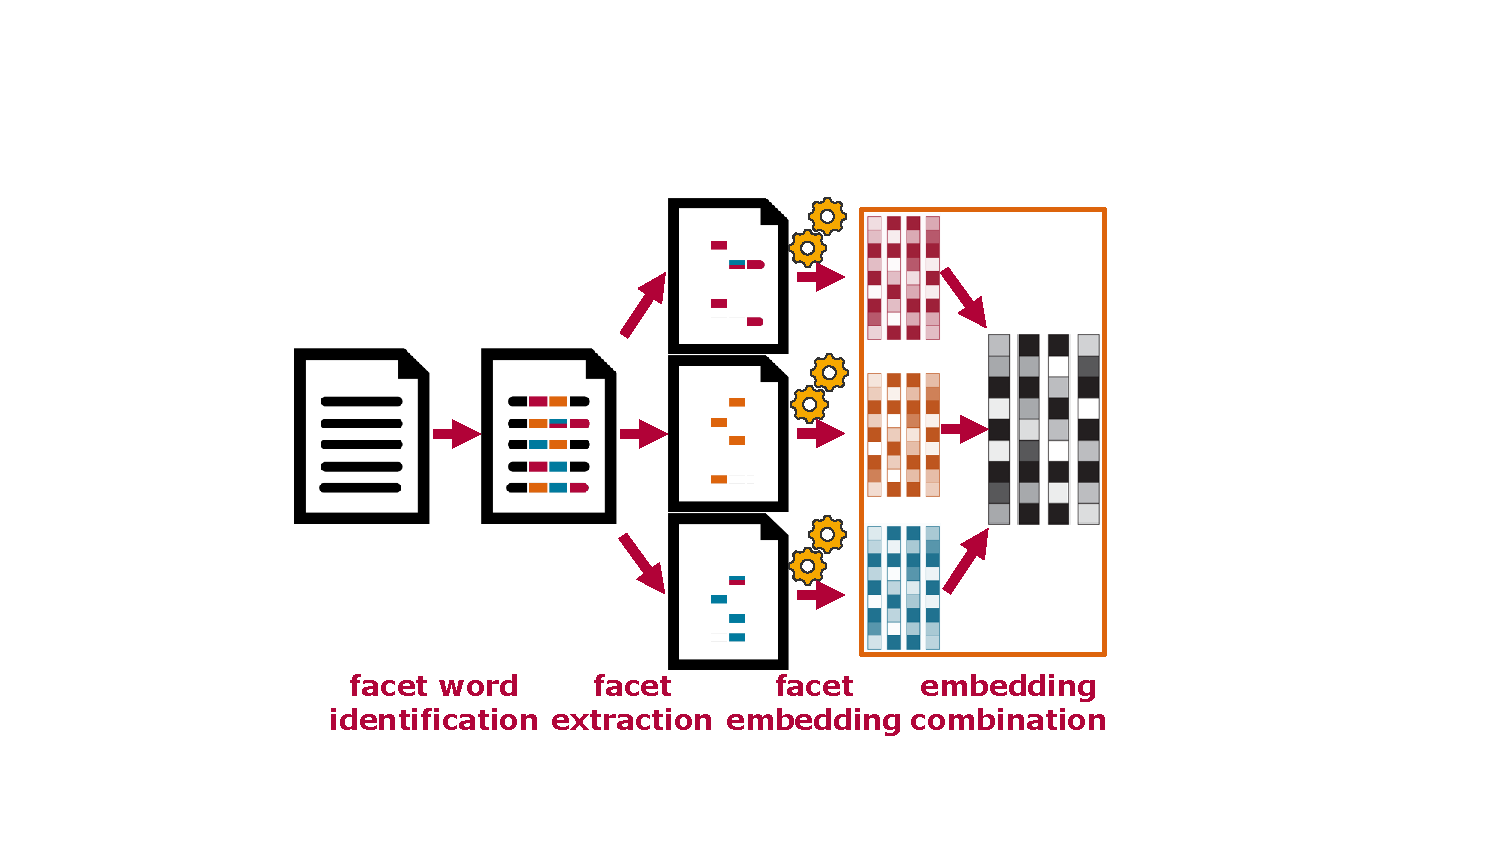
\includegraphics[width=0.99\linewidth]{figures/approach_overview.pdf}
	\caption{Overview of the four main processing steps of \emph{lib2vec}.}
   \label{fig:overview}
\end{figure}

Embeddings for long documents are typically realized by splitting them into smaller parts following either a truncation-based, chunk-based, or a facet-based strategy.
Truncation-based approaches are using only the first $n$ words of a text, where $n$ corresponds to the input sequence limit of the embedding algorithm.
%As a downside, most of the words in a book are not used to obtain a representation, which can result in a poor embedding quality.
Chunk-based approaches split a text into several segments of size $n$ with $n\leq$ input sequence limit.
Then, each segment is embedded separately and then combined, for example via summation.
%Despite the complete full-text can be considered with the chunk-based strategy, a downside could be an increased calculation time because more data need to be processed.
%Furthermore, all books could consist of different numbers of chunks, which leads to less flexibility and more information loss during the combination of chunks.
%A consequence of this information loss is a poor quality of the obtained embedding.
Both these strategies loose crucial information either by ignoring large parts of the text (truncation) or by averaging intermediate results (chunking).
To overcome thes disadvantages, we propose \emph{lib2vec} which follows the idea by \citet{risch_book_2018} and divides a text into several facets, instead of chunks.
The novel core idea of \emph{lib2vec} is to split long texts not sequencially based on document position but rather selectively based on semantic facets

We define facets as subsets of words following semantic categories.
In this work, these categories are oriented toward the perspectives of literary analysis such as atmosphere or style.
Thereby, each category includes certain words, for example, the style facet includes stopwords since there usage is a good indicator for different styles.
Besides, words that appear in one facet may also appear in another facet.
Compared with truncation-based approaches, facet-based approaches make use of more words of a text.
While the number of chunks differs for each text, the number of facets is constant for any text.
In addition, facets are semantically meaningful, while chunks only provide information about the position within a text.

\subsection{Processing Pipeline of lib2vec}

Figure~\ref{fig:overview} illustrates the overall concept for our multi-faceted embedding approach: identifying candidate words, constructing pseudo-documents, and computing embeddings.

\paragraph{Facet Word Identification.}
In the first step, documents are preprocessed with sentence splitting, tokenization, lemmatization, POS-tagging, named entity recognition (NER), and semantic word dictionary lookups.
Each book in a corpus is annotated automatically, using SpaCy~\citep{honnibal2020spacy}, Heideltime~\citep{stroetgenmultilingual2013}, the German semantic dictionary GermaNet~\citep{hamp1997germanet, henrich2010gernedit}, and the English semantic dictionary WordNet~\citep{fellbaum2010wordnet}.
%While SpaCy extracts sentences, tokenizes texts, lemmatizes words, and assigns POS- and NER-tags, Heideltime is specialized for temporal named entities.
%GermaNet and WordNet identify abstract place, time, and atmosphere descriptors for the \emph{lib2vec} extensions \textit{Net} and \textit{Net Only}.
%While the Net extension combines these descriptors with POS-tags and named entities, the Net Only variant exclusively utilizes the semantic dictionaries.

\paragraph{Facet Extraction.}
In this step, words in a document are assigned to none, one, or multiple of the facets \textit{time}, \textit{place}, \textit{style}, \textit{atmosphere}, \textit{plot} or \textit{content}.
Additional facets can be defined in the future if necessary.
%Previous annotations are used to identify and assign facet words.
%In some cases, the actual context of a selected word may be lost. 
%This loss of context can cause problems in context-sensitive embedding algorithms.
%To preserve the context, an additional word window of length $w$ can be added around the actual facet word to the set of the facet words.
%Preserving the context by this mechanism is referred to as \textit{window extension}.
For each facet, a pseudo-document is generated containing all assigned words.
%In order to find the correct numeric encoding for a specific facet of a document, a unique identifier is created for each pseudo-document.
%The identifier contains the original document identifier as well as an identifier for the represented facet.
%Thus, the created identifier enables the individual targeting of document facets for all books.

\paragraph{Facet Embedding.}
Each pseudo-document consists of only a fraction of the words of the original book.
This allows to compute facet-specific embeddings using existing document embedding approaches.
%To encode a facet, which means, to encode the pseudo-document constructed of the associated facet-words, the pseudo-document is passed to an embedding algorithm.
%In other words, the embedding algorithm processes all facet-based pseudo-documents instead of the original full-texts.
%Compared with truncation-based algorithms, \emph{lib2vec} can use more words of the full-text.
%The number of documents, as well as the number of words that the algorithm has to process, is thus increased.
%Since the algorithm has more data available, this increase can already improve the quality of the results.
%Theoretically, any document embedding algorithm can be used in this step.
We opted for using doc2vec since it has the largest input sequence limit.
In case the pseudo-document exceeds this limit, the facet is truncated.
%Alternatively, instead of truncation, the facet can be chunked.

\subsection{Facet Definitions}
As described earlier, we use the tagged documents to construct pseudo-documents for each facet.
In this section, we describe in more detail how these pseudo-documents are compiled.

\paragraph{Location.}
The location facet is based on tokens that are tagged as geopolitical locations and buildings by SpaCy NER.
%This is a major difference to \citet{risch_book_2018}, who obtained an averaged vector of pre-trained embeddings of location words.
Multiple appearances of a word are kept to preserve their frequency, as intermittently reappearing places may be more important to the book.
%The same applies to other facets as well.
A downside of NER is, that unnamed places such as \textit{ocean}, \textit{garden}, or \textit{street} are not included.
Thus, we use GermaNet or WordNet to identify location descriptors.
%GermaNet and WordNet contain specific groups of words, for example, \textit{location} or \textit{emotion}.
%Each lemmatized word form in these groups is added to the pseudo-document if it occurs in the current book text for the \textit{Net} and \textit{Net Only} variants.

\paragraph{Time.}
Similar to location, we use NER to construct the pseudo-document for the time facet.
Although this covers months, seasons, or year numbers, phrases referring to historical events such as revolutions or wars are not tagged by standard NER tools.
Thus, we again utilise  GermaNet or WordNet to extend the scope to include events and abstract time descriptors.

\paragraph{Style.}
Prior studies have shown correlations between authorship attribution, the style of a text, and the usage of stopwords~\citep{arun_stopword_2009, tausczik_psychological_2010, alharthi_authorship_2018}. 
Following these findings, we construct the style facet based on all stopwords found by a POS-tagger.
Since stopwords appear very frequently, we expect this pseudo-document to grow quickly.
Although this might be problematic considering sequence length limitations of embeddings, we assume that truncated stopwords are already present in the limited sequence and the potential loss of information is small.

\paragraph{Atmosphere.}
Adjectives and adverbs are common linguistic indicators of the atmosphere of a text, since they describe the properties of objects, people, or emotions.
In addition, affective or sensual words such as \textit{gloomy}, \textit{warm}, \textit{smell}, or \textit{howl} also have a great influence on the atmosphere~\citep{tausczik_psychological_2010}.
In order to take these affective and sensual words into account, we consider nouns, verbs, and adjectives corresponding to emotions and feelings as identified by GermaNet or WordNet.

\paragraph{Plot.}
We utilise the basic assumption that the plot of a novel describes the actions between characters~\citep{labatut_extraction_2019, lee_story_2020}.
Such actions are expressed by verbs and adverbs.
Thus, we construct the pseudo document for the plot facet based on words with these POS-tags.

\paragraph{Content.}
We use topic modelling to construct the pseudo-document for the content facet.
Topic modelling has been shown to be useful for analyzing literary texts~\citep{uglanova_2020}.
Due to its high computational costs, we only include this facet for the book comparison task (Section~\ref{ssec:bookComparisons}.
We trained an LDA~\citep{blei2003latent} topic model on the input corpus and set the number of topics to 15.
Afterwards, we use the top 100 associated words of the five most relevant topics of a book according to the inferred topic distribution.
Given that topic modelling plays only a minor part in \emph{lib2vec} we treat it as a black box and defer furhter analysis to future work.

\paragraph{Raw.}
In addition, we also include a full-text facet containing the beginning of a book without any filtering apart from the truncation after the maximum sequence length.
In contrast to other facets, the raw facet preserves continuous text and word order which may improve the results if the applied document embedding algorithm can take advantage of such textual continuities.


\subsection{Combination of Facets}

In the previous sections we described the construction of pseudo-documents for facets.
For practical reasons and in order to compare our approach to other document embedding methods, we need to combine the facet embeddings into a single vector.
\citet{rettig_fusing_2019} cover a number of approaches of aggregating embedding vectors for their multi-faceted word embeddings.
The na\"ive approach to combine facet embeddings is to use the arithmetic mean (AVG) or an element-wise sum of the individual vectors.
\citet{gittens_skip-gram_2017} have empirically shown that the summation of word and document embeddings can retain aspects of two underlying embedding vectors.
Another approach is to simply concatenate facet embedding vectors (CONCAT).
This has the advantage that facet embeddings can have a different dimensionality and the information captured by each facet is still available in the resulting vector.

We propose to combine concatenation with dimensianality reduction to benefit from more encoded information while keeping the dimensionality low.
To this end, we used principal component analysis on the concatenated vectors (PCA).
We also experimented with other dimensionality reduction methods, such as autoencoders, but results were worse compared to the PCA.
And PCA has the advantage, that it can be computed very efficiently.
However, projecting previously unseen books into the low-dimensional space is not easily possible.
Another downside of dimensionality reduction in general is that a rather large corpus is necessary to identify the latent dimensions. 
Furthermore, the resulting embeddings cannot be used for semantic operations using facet encodings.
In the experiments, we report results for three different combination methods: AVG, CONCAT, and PCA.

\section{Experimental Setup}

In this section we provide an overview of which datasets we use for our evaluation, how we mitigate the influence of potential biases in our experiments, and describe the baselines we compare our approach to.

\subsection{Datasets}

%\renewcommand{\tabcolsep}{3.7pt}
%\begin{table}
%	\centering
%	\footnotesize
%	\begin{tabular}{L{0.87cm}L{0.64cm}R{0.63cm}R{0.76cm}R{0.77cm}R{0.71cm}R{0.7cm}R{0.65cm}}
%		\toprule
%		Dataset & Language & \# Books & \# Words & \# Unique Words & $\varnothing \#$ Words per Book  & $\varnothing \#$ Unique Words per Book & $\varnothing \#$ Books per Author \\
%		\midrule
%		CGF    & GER      & 3.2K    & 204M            & 26M       & 46K          & 7.2K                    & 5.7                \\
%	%	S-CGF  & GER      & 208      & 22.2M          & 2.63M      & 81.4K         & 11.1K                    & 4.24                \\
%		DTA    & GER      & 459      & 26M           & 4M        & 44K         & 7.5K                    & 2.1                \\
%%		LitRec & EN       & 3.1K    & 275M            & 22M       & 73K          & 7.0K                    & 2.8                \\
%		MGG    & EN       & 1K       & 17M           & 3M        & 17K         & 2.8K                    & 2.1                \\
%		BoCo    & EN       & 20       & 4M             & 198K    & 145K             & 8.9K                    & 1.2       \\
%		\bottomrule
%	\end{tabular}
%	\caption[Overview of Different Dataset Characteristics]{Overview of dataset characteristics.
%		The number of books for each corpus and its language, values for word counts and vocabulary sizes are reported. The median is reported for the amount of words per book and the mean for the amount of books per author.}
%	\label{tab:datasets_overview}
%\end{table}

\begin{table}
	\centering
	\begin{tabular}{crrrr}
		\toprule
		Dataset                                			& CGF  & DTA  & MGG  & BoCo  \\
		\midrule
		$\text{Language}$                               	& GER  & GER  & EN   & EN   \\[0.2em]
		$\text{\# Books}$                               	& 3.2K & 459  & 1K   & 20   \\[0.2em]
		$\text{\# Words}$                               	& 204M & 26M  & 17M  & 4M   \\[0.2em]
		$\text{\# Unique Words}$                        	& 26M  & 4M   & 3M   & 198K \\[0.2em]
		$\frac{\text{\# Words}}{\text{per Book}}$	 	& 46K  & 44K  & 17K  & 145K \\[0.2em]
		$\frac{\text{\# Unqiue Words}}{\text{per Book}}$	& 7.2K & 7.5K & 2.8K & 8.9K \\[0.2em]
		$\frac{\text{\# Books}}{\text{per Author}}$     	& 5.7  & 2.1  & 2.1  & 1.2  \\
		$\frac{\text{\# Books}}{\text{per Series}}$     	& 2.5  & 3.2  & --  & --  \\
		\bottomrule
	\end{tabular}
	\caption[Overview of Dataset Characteristics]{Overview of dataset characteristics}
	\label{tab:datasets_overview}
\end{table}

Key characteristics of the datasets used are provided in Table~\ref{tab:datasets_overview}.
The median is reported for the average number of (unique) words per book and the mean for the average number of books per author.

\paragraph{Corpus of German-Language Fiction (CGF).}
The Corpus of German Fiction by~\citet{fischer_corpus_2017} consists of \numprint{3219} German prose books published between 1840 and 1930.
%The vast majority of books (\numprint{2735}) were written by 549 German authors, the others are translated into German as they were originally published in by 18 English, Russian, and French authors.
For our series classification task, we identified \numprint{208} books that were part of a series or sequels.
%To select books that belong to the same book series, we use indicator words of the title, such as \textit{Band}, (\textit{volume}) or \textit{Teil} (\textit{Part}).
%In most cases, books in the same series have the same title but a specific series number.

\paragraph{Deutsches Text Archiv (DTA).}
The DTA corpus contains \numprint{765} German works of belles-lettres published between the 16th and 20th century~\citep{berlin-brandenburgischen_akademie_der_wissenschaften_deutsches_2021}.
We exclude texts published before 1800, as German language has changed significantly since then, leaving \numprint{459} texts.
In this corpus, we were able to identify \numprint{176} books which are part of a series.
%\paragraph{LitRec.}
%LitRec is a dataset that contains full-texts of English books from Project Gutenberg~\citep{vaz_litrec_2012}.
%The \numprint{3458} full-texts written by \numprint{1109} authors.
%This dataset was annotated with \numprint{35507} ratings by book readers.

\paragraph{Gutenberg and Genres (MGG).}
\citet{maharjan_multi-task_2017} created the MGG corpus consisting of \numprint{1003} full-texts of English books to evaluate success and genre prediction methods. 
%This corpus by~\citet{maharjan_multi-task_2017} contains \numprint{1003} full-texts of English books and was built to evaluate book models within success and genre prediction tasks. 
It contains genre information and binary labels of success based on Goodreads ratings. 
A book is labeled successful if it has an average rating of more than 3.5 stars from at least ten people.

\paragraph{Book Comparison (BoCo).}
This dataset consists of 20 popular English books selected from Project Gutenberg.\footnote{\url{www.gutenberg.org}}
We conducted a survey with 81 participants who were asked to asses which two books in a triplet of books are more similar with regard to when and where they are set, as well as their atmosphere, content, plot and overall similarity. 
In total, we were able to gather ratings on 527 triplets with an moderate annotator agreement of a Fleiss' Kappa Score of 0.55.

\subsection{Removal of Possible Biases}

In preliminary experiments we saw a significant correlation between the length of a texts and the similarity score for doc2vec and average word2vec representations.
Our \emph{lib2vec} approach was far less affected by the length of books.
Nevertheless, to allow for a fair comparison between approaches, we run all experiments with books of comparable length to exclude length as a distinguishing feature.

For experiments on identifying series of books or books by the same author, we remove words that may provide a clear distinction.
For example, character names of a sequel may not appear in other books and thus render identifying books of the same series a trivial task.
We remove words with a document frequency below a threshold based on each dataset.
Although this significantly reduces the size of the overall vocabulary, document length distributions are barely affected.

\subsection{Baselines}

We compare \emph{lib2vec} to various traditional and state-of-the-art baselines.
As the most simple baseline, we choose a bag-of-words (BoW) representation limited to a vocabulary size of \numprint{30000} words.
Furthermore, we use standard word2vec embeddings trained on each corpus.
We calculate the arithmetic mean of all words in a book to get a single vector representation for the book.
In addition, we compute representations of books using doc2vec~\cite{le_distributed_2014}.
Preliminary experiments with pre-training the doc2vec model yielded worse results, therefore we train the doc2vec model on each corpus seperately.
We also use more recently published models, namely BERT~\citep{devlin_bert_2019}, RoBERTa~\citep{liu2019roberta}, XLM~\citep{conneau2019cross}, fine-tuned for sentence representation by SentenceTransformers~\citep{reimers-2019-sentence-bert}.
These approaches are limited by the maximum sequence length, however \citet{khalifa_will_2020} have shown that the first 1,000 sentences can be sufficient to encode books.
Additionally, we use the partitioned word averaging model P-SIF~\citep{gupta_p-sif_2020} as a state-of-the-art document embedding algorithm which is designed partiularly for long documents.

\section{Evaluation}

We evaluate our approach on various tasks.
Due to space constraints, we limit the results presented here to the setup that performed best for each approach.
More details can be found in the appendix.
For all experiments, we only use the documents of each corpus to train the doc2vec embedding for each facet for our approach.
In constrast to models such as BERT, which need to be trained on millions of tokens, \emph{lib2vec} achieves very good results with only a fraction of training data.

\subsection{Book Similarities}
%\begin{table*}
%	\centering
%	\begin{tabular}{l|ccccc|ccc|c} % TODO fix the bold results
%		\toprule
%		                 &           DTA &         DTA-L &         DTA-M &        DTA-Sh &         CGF-L &           CGF &          CGF-M &          CGF-Sh & MGG \\ \midrule
%		\textbf{Author}  &               &               &               &               &               &               &                &                 &  \\
%		BoW              &          0.69 &          0.81 &          0.78 &          0.68 &          0.69 &          0.67 &           0.61 &          0.57   & 0.53\\
%		AVG W2V          &          0.67 &          0.81 &          0.68 &          0.74 &          0.64 &          0.65 &           0.57 &          0.58   & 0.51\\
%		doc2vec          & \textbf{0.74} & \textbf{0.89} & \textbf{0.78} & \textbf{0.79} & \textbf{0.74} & \textbf{0.75} &  \textbf{0.73} & \textbf{0.70}   & 0.69\\
%		BERT             &          0.40 &          0.42 &          0.30 &          0.39 &          0.51 &          0.60 &           0.51 &          0.60   & 0.43\\
%		RoBERTa          &          0.38 &          0.37 &          0.30 &          0.39 &          0.43 &          0.55 &           0.44 &          0.50   & 0.42\\
%		XLM              &          0.38 &          0.37 &          0.31 &          0.38 &          0.48 &          0.58 &           0.49 &          0.53   & 0.42\\
%		P-SIF            &          0.66 &          0.77 &          0.73 &          0.63 &          0.69 &          0.68 &           0.61 &          0.61   & 0.55\\
%		lib2vec AUTO     & \textbf{0.80} &          0.92 & \textbf{0.86} & \textbf{0.86} &          0.93 &          0.86 &           0.88 &          0.79   & 0.66\\
%		lib2vec PCA      &          0.79 &          0.92 &          0.85 &          0.78 & \textbf{0.96} & \textbf{0.89} &  \textbf{0.92} &          0.79   & 0.71\\ \midrule
%		\textbf{Series}  &               &               &               &               &               &               &                &                 & \\
%		BoW              &          0.92 &          0.86 &          0.83 & \textbf{0.90} &          0.74 & \textbf{0.80} &  \textbf{0.80} &          0.44   & -- \\
%		AVG W2V          &          0.89 &          0.86 &          0.76 & \textbf{0.90} &          0.66 &          0.64 &           0.63 &          0.37   & -- \\
%		doc2vec          & \textbf{0.94} & \textbf{0.88} & \textbf{0.83} & \textbf{0.90} & \textbf{0.76} &          0.77 &           0.76 &          0.44   & -- \\
%		BERT             &          0.39 &          0.42 &          0.29 &          0.45 &          0.66 &          0.64 &           0.58 &          0.43   & -- \\
%		RoBERTa          &          0.34 &          0.36 &          0.29 &          0.45 &          0.41 &          0.40 &           0.38 &          0.32   & -- \\
%		XLM              &          0.36 &          0.37 &          0.30 &          0.45 &          0.56 &          0.54 &           0.47 &          0.32   & -- \\
%		P-SIF            &          0.89 &          0.86 &          0.79 &          0.85 &          0.69 &          0.70 &           0.69 &          0.37   & -- \\
%		lib2vec AVG      &          0.95 &          0.91 &          0.84 & \textbf{0.90} &          0.82 &          0.86 &           0.80 &          0.30   & -- \\
%		lib2vec PCA      & \textbf{0.98} &          0.92 &          0.85 & \textbf{0.90} &          0.84 &          0.87 &           0.79 &          0.30   & -- \\ \bottomrule& 
%	\end{tabular}
%	\caption[Author and Series Task Results of Baselines and lib2vec Variants]{Author (A) and Series (S) Task NDCG scores of baseline and different combination variants of lib2vec with strict specific word filter on different corpora and short (Sh), medium (M) and large (L) length specific sub-corpora. The highest values for each task and dataset are highlighted in bold.}
%	\label{tab:ndcg_multi}
%\end{table*}
\begin{table}
	\centering
	\tabcolsep=1.3pt
	\begin{tabular}{lcccccccc}
		\toprule
		                             &        \multicolumn{3}{c}{Author}        &  & \multicolumn{2}{c}{Series} & & Genre\\ \cmidrule{2-4}\cmidrule{6-7}\cmidrule{9-9}
		                             &      DTA      &   CGF    	 &     MGG       &   &     DTA       &   CGF   & &   MGG    \\ \midrule
		BoW                          &     0.18   	 &   0.28   	 &     0.13      &   &     0.31      &  0.18      	 & &   0.44 \\
		AVG W2V                      &     0.17      &   0.26   	 &     0.12      &   &     0.31      &  0.15      	 & &   0.50 \\
		doc2vec                      &     0.21      &   0.43   	 &     0.22      &   &     0.31      &  0.18      	 & &   0.50 \\
		BERT                         &     0.04      &   0.19   	 &     0.05      &   &     0.09      &  0.13      	 & &   0.34 \\
		RoBERTa                      &     0.04      &   0.06    	 &     0.04      &   &     0.06      &  0.06      	 & &   0.29 \\
		XLM                          &     0.04      &   0.11    	 &     0.05      &   &     0.07      &  0.09      	 & &   0.34 \\
		P-SIF                        &     0.17      &   0.31    	 &     0.14      &   &     0.30      &  0.17      	 & &   0.52 \\
		\emph{lib2vec} AVG           &     0.22      &   0.53    	 & \textbf{0.23} &   &     0.31      &  0.19      	 & &   0.55 \\
		\emph{lib2vec} CON           & \textbf{0.23} & \textbf{0.62} &     0.20      &   & \textbf{0.32} &  0.19	  	 & &   0.79 \\
		\emph{lib2vec} PCA           & \textbf{0.23} & 	 0.61        &     0.20      &   & 	   0.31 	 & \textbf{0.20} & &   \textbf{0.80} \\
		Upper bound                  &     0.31      &   0.74        &     0.34      &   &     0.32      &  0.21      	 & &   1.00 \\ \bottomrule
	\end{tabular}
	\caption{Precision@k for author, series, and genre task using cosine similarities of different embedding models. Scores closest to upper bound are highlighted in bold.}
	\label{tab:sim}
\end{table}

%\begin{table}
%	\centering
%	\begin{tabular}{lcc}
%		\toprule
%		                   &    Prec@10    &    Rec@10     \\ \midrule
%		BoW                &     0.44      &     0.05      \\
%		AVG W2V            &     0.50      &     0.05      \\
%		doc2vec            &     0.50      &     0.05      \\
%		BERT               &     0.34      &     0.04      \\
%		RoBERTa            &     0.29      &     0.03      \\
%		XLM                &     0.34      &     0.04      \\
%		P-SIF              &     0.52      &     0.05      \\
%		\emph{lib2vec} AVG &     0.55      &     0.06      \\
%		\emph{lib2vec} CON &     0.79      & \textbf{0.08} \\
%		\emph{lib2vec} PCA & \textbf{0.80} & \textbf{0.08} \\ \bottomrule
%	\end{tabular}
%	\caption{Genre task using cosine similarities of different embedding models on MGG dataset. Best scores highlighted in bold.}
%	\label{tab:genre}
%\end{table}

As a first experiment, we use an information retrieval setting to measure how well embeddings encode similarities of books from the same author, same genre, and same book series.
For each book, we look at the 10 nearest neighbors in the respective embedding space and compute precision@10 for the three tasks (see Table~\ref{tab:sim}.
Note that not all datasets have series or genre annotations and are therefore excluded for some of the experiments.
Given that we do not have 10 positive examples for all tasks and classes, we also report the upper bound of maximal achievable precision@10.
Our \emph{lib2vec} embedding consistently performs best and significantly outperforms state-of-the-art embeddings as well as traditional vector representations.
For the genre classification task, we use the MGG corpus (the others don't contain genre annotations).

\subsection{Book Comparisons}\label{ssec:bookComparisons}

\begin{table*}
	\centering
	\begin{tabular}{lccccccc}
		\toprule
		Algorithm          &     Total     &     Time      &   Location    &     Plot      &  Atmosphere   &    Content    &   Micro AVG   \\ \midrule
		BoW                &     0.46      &     0.46      &     0.49      &     0.46      &     0.48      &     0.48      &     0.47      \\
		AVG W2V            &     0.47      &     0.59      &     0.46      &     0.46      &     0.42      &     0.41      &     0.46      \\
		BERT               & \textbf{0.63} &     0.57      & \textbf{0.55} &     0.57      & \textbf{0.58} & \textbf{0.57} &     0.58      \\
		RoBERTa            &     0.50      &     0.39      &     0.45      &     0.49      &     0.50      &     0.52      &     0.48      \\
		XLM                &     0.40      &     0.36      &     0.43      &     0.47      &     0.41      &     0.43      &     0.42      \\
		P-SIF              &     0.35      &     0.42      &     0.41      &     0.38      &     0.37      &     0.39      &     0.39      \\
		\emph{lib2vec} AVG &     0.62      & \textbf{0.64} &     0.54      & \textbf{0.59} & \textbf{0.58} &     0.55      & \textbf{0.59} \\
		\emph{lib2vec} CON &     0.47      &     0.49      &     0.46      &     0.38      &     0.40      &     0.48      &     0.46      \\
		\emph{lib2vec} PCA &     0.57      &     0.55      &     0.49      &     0.47      &     0.52      &     0.51      &     0.52      \\ \bottomrule
	\end{tabular}
	\caption[Precision of Baselines and \emph{lib2vec} on {BoCo}]{Precision of baselines and \emph{lib2vec} on the {BoCo} dataset. 
		Words that only occur in three or fewer documents are removed (strict specific word filter).
		The performance within the specific similarity types is expressed as the ratio of correctly predicted most similar neighbors and all triplets for different algorithm configurations. Micro AVG represents the ratio of all correct predictions and all assessments.
		The other similarity types refer to their respective facets.}
	\label{tab:book_comparison_baselines_strict}
\end{table*}

In the previous experiment we evaluated the different embeddings with respect to metadata associated with each book.
To evaluate the facets more directly, we created the BoCo dataset containing manual book similarity annotations with respect to different aspects.
Each expert rated which two books out of a set of three books are more similar to each other with respect to when and where the story is set (time, location), as well as their plot, atmosphere, content and overall (total) similarity.
Each triplet has multiple annotations and we use the majority vote in cases where the annotators disagreed.

Table~\ref{tab:book_comparison_baselines_strict} lists the precision of different models regarding the agreement with human annotators.
We consider only precision because the annotations do not provide information about false negatives which are required for recall.
In order to rate the similarity, we use the respective document embeddings and calculate the cosine similarity between the three books in a given triplet.
We then count for how many triplets a model agrees with the human annotations.
For \emph{lib2vec}, we use facet embeddings where applicable.
Surprisingly, traditional embeddings and even bag-of-words are able to beat state-of-the-art transformer model P-SIF, which was especially designed for long texts.
Overall, BERT and \emph{lib2vec} perform best and yield very similar results across all facets.

\subsection{Document Classification}

\begin{table}
	\centering 
	\begin{tabular}{lrr}
		\toprule
		Algorithm                        &        Rating &         Genre \\ \midrule
		\citet{maharjan_multi-task_2017} & \textit{0.72} &            -- \\
		\citet{khalifa_will_2020}        & \textit{0.72} &            -- \\ \midrule
		BoW                              &          0.61 &          0.19 \\
		AVG W2V                          &          0.70 &          0.59 \\
		doc2vec                          &          0.71 &          0.56 \\
		BERT                             &          0.70 &          0.49 \\
		RoBERTa                          &          0.69 &          0.41 \\
		XLM                              &          0.71 &          0.47 \\
		P-SIF                            &          0.70 &          0.55 \\
		\emph{lib2vec} AVG               &          0.72 &          0.63 \\ 
		\emph{lib2vec} CON               & \textbf{0.76} & \textbf{0.89} \\
		\emph{lib2vec} PCA               &          0.69 &          0.56 \\ \bottomrule
	\end{tabular}
	\caption{Weighted F1 scores for classification of high-rated books and genres using RBF-based SVM on different book embeddings on MGG. The largest values are highlighted in bold. Italic values were taken from the corresponding publications.}
	\label{tab:down_stream_eval_f1}
\end{table}

We also evaluate the performance of different embeddings in a document classification setting as a downstream application.
The MGG dataset~\citep{maharjan_multi-task_2017} contains information about high-rated books.
We use the same binary classification setup as \citep{maharjan_multi-task_2017} and \citep{khalifa_will_2020}, which uses the weighted F1-score to measure performance.
Using book representation baselines and our \emph{lib2vec} embedding, we train an SVM with RBF-kernel on the LitRec dataset~\citep{vaz_litrec_2012}.
It contains \numprint{3458} full-texts of English books written by \numprint{1109} authors from Project Gutenberg which were rated by \numprint{35507} users.
Table~\ref{tab:down_stream_eval_f1} shows the classification performance for rating and genre prediction.
The classifier using our \emph{lib2vec} embedding is able to outperform all baselines as well as the approaches from related work which are especially tailored toward this task.
%Besides, we repeated the task with the available genre labels and outperformed all baselines.

\subsection{Qualitative Evaluation}

\begin{figure*}[h]
	\centering
	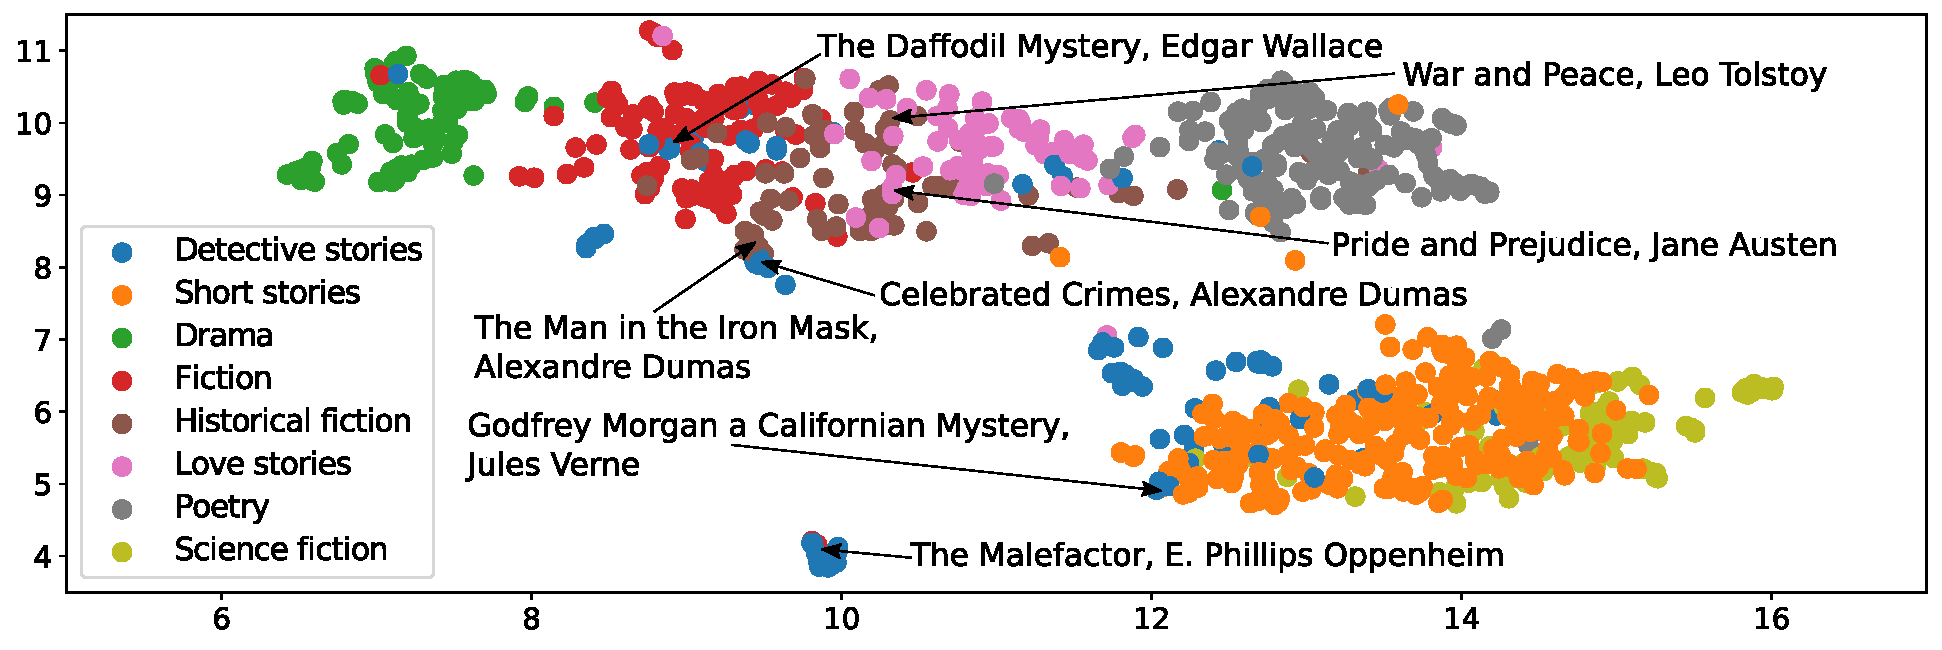
\includegraphics[width=\textwidth]{figures/plot_genres_multi_column.pdf}
	\caption{UMAP projection of the facet \textit{plot} of \emph{lib2vec} trained on the MGG corpus.}
	\label{fig:plot_genres_multi_column}
\end{figure*}

We also performed an extensive qualitative evaluation of the \emph{lib2vec} model with respect to aggregated representation and individual facet embeddings in collaboration with domain experts from literary sciences.
Figure~\ref{fig:plot_genres_multi_multi_column} depicts a UMAP visualization of the embedding space of the plot facet for the MGG corpus. The different colors indicate the genre of the novels.
Note that the plots of the detective stories is scattered across multiple genre clusters and that,e.g., historical fiction has some overlap with love stories.


\section{Conclusions \& Future Work}

Traditional embedding algorithms have an input sequence limit for the efficient encoding of documents.
Long texts, such as novels, often exceed these limits.
Therefore, not all available information is used when embedding long documents, or the long documents are split sequencially into smaller chunks.
Both solutions result in sub-optimal performance on a variety of tasks regarding long documents.
We introduced \emph{lib2vec}, a multi-faceted document embedding framework that splits long documents not sequencially but semantically based on domain-specific facets.
It provides semantically more meaningful document representations than truncation- or chunk-based methods.
%We were able to show the effectiveness of our approach in several experiments.
%Due to the lack of benchmark datasets, we conducted a survey on book similarities to create the BoCo dataset.
%Aside from that, we also used meta-data, such as series associations, author names, and genre labels.
Our approach outperforms baselines, such as doc2vec, BERT, or P-SIF for corpora that contain large- and medium-sized novels on classification tasks, rating prediction, and assessing similarities.
%However, \emph{lib2vec} was not able to exceed the performance of traditional and state-of-the-art embeddings on shorter documents.
%We have also shown that our model outperforms others in classification tasks, such as predicting high-rated books.

The most interesting question for future work is how to incorporate additional knowledge into our model, e.g., by pre-training and/or fine-tuning.
Large language models encode semantic knowledge that we aim to utilize for facet computation in the future.
We further want to test \emph{lib2vec} in other domains with other facets, e.g., for long scientific texts, or legal documents.
Also, in the literary domain, there are facets we didn't explore yet, such as readability~\cite{feng_2010} or literariness~\cite{van_2019}.




%We encourage you to use the natbib styles.
%You can use the command \verb|\citet| (cite in text) to get ``author (year)'' citations, like this citation to a paper by \citet{Gusfield:97}.
%You can use the command \verb|\citep| (cite in parentheses) to get ``(author, year)'' citations \citep{Gusfield:97}.
%You can use the command \verb|\citealp| (alternative cite without parentheses) to get ``author, year'' citations, which is useful for using citations within parentheses (e.g. \citealp{Gusfield:97}).

%Unicode cannot be used in Bib\TeX{} entries, and some ways of typing special characters can disrupt Bib\TeX's alphabetization. The recommended way of typing special characters is shown in Table~\ref{tab:accents}.
%
%Please ensure that Bib\TeX{} records contain DOIs or URLs when possible, and for all the ACL materials that you reference.
%Use the \verb|doi| field for DOIs and the \verb|url| field for URLs.
%If a Bib\TeX{} entry has a URL or DOI field, the paper title in the references section will appear as a hyperlink to the paper, using the hyperref \LaTeX{} package.

% Entries for the entire Anthology, followed by custom entries
\bibliography{anthology,custom}
\bibliographystyle{acl_natbib}

\clearpage
\appendix


\section{Reader Survey}
\label{appendix:survey}
\begin{table}
	\centering
%	\footnotesize
	
	\begin{tabular}{lR{1cm}rrrr}
		\toprule
		Language & \# Participants &	Mean    & STD    & Min & Max \\
		\midrule
		ENG      &  9			& 10.44 & 4.32 & 6   & 19  \\
		GER      & 	72			& 7.93  & 4.52 & 0   & 19 \\
		ALL      &  81			& 8.21  & 4.56 & 0   & 19  \\
		\bottomrule
	\end{tabular}
	\caption[Knowledge Distribution Characteristics]{Knowledge distribution characteristics. 
		The mean, the standard derivation, the minimum and the maximum values of known books are reported for English and German language groups.}
	\label{tab:known_books}
	% Verweis im Text mittels \ref{tbl:beispieltabelle}
\end{table}

\begin{figure*}
	\centering
	\fbox{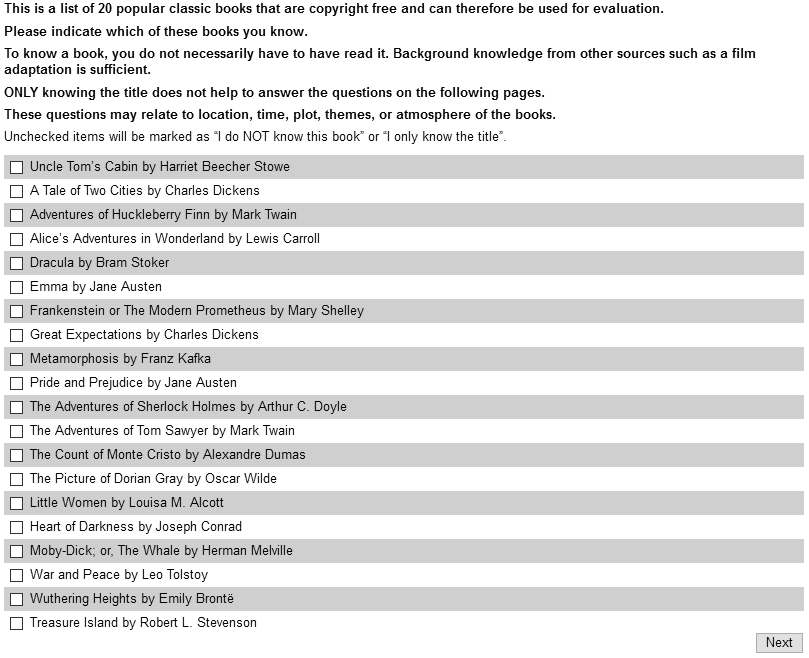
\includegraphics[width=\linewidth]{figures/survey1}}
	\caption{Overview of the first part of the reader survey. Participants can select books they know.}
	\label{fig:survey1}
\end{figure*}

The online survey started on 26th January and ended on 26th March 2021.
It offered German and English questions to allow participation for as many volunteers as possible.
81 experts and students of English, German or general literary studies participated.
They were invited through e-mail distribution lists to which they were subscribed, in consultation with the responsible persons for the distribution list.
Nine participants knew two books or fewer, three participants knew only one book triplet that is not included in the survey, and one person knew five books, none of which occur together as a triple.
In total, the assessments of 68 experts could be used.
Table~\ref{tab:known_books} shows characteristics for the knowledge distribution.
On average, the participants who selected the English language for the survey had known more books than the German participants.
Besides, the nine English-speaking participants knew at least six books.

The survey consisted of two parts.
In the first part, readers had to decide which books from BoCo they know.
BoCo contains freely available and popular books, where popularity is measured in the download numbers of Project Gutenberg in December 2020.
By focusing on popular books, more people were able to participate in the study.
From the top-100 downloaded books, 20 books are selected manually by an expert based on familiarity levels to reduce the number of items for the first part of the survey.

\begin{figure*}
	\centering
	\fbox{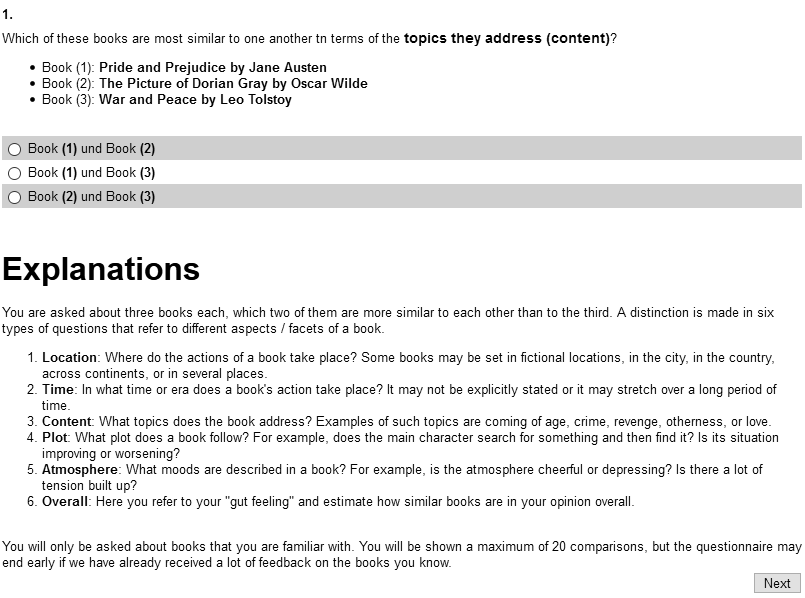
\includegraphics[width=\linewidth]{figures/survey2}}
	\caption{Overview of the second part of the reader survey. Participants have to decide which two books are more similar from a triplet of books for a specific similarity type.}
	\label{fig:survey2}
\end{figure*}

Figure~\ref{fig:survey1} shows the selected books for BoCo in the first part of the survey.

After the participants rated the books they know, they have been confronted with the following task illustrated by Figure~\ref{fig:survey2} in the second survey part.
For three known books, the participants had to assess the most similar book pair for a single similarity category such as location, time, atmosphere, topic, plot, and overall similarity.
These similarities corresponded to a large extent to the facets described in our paper, but only those were selected for which one does not currently need to have the book text available. 
The writing style was therefore excluded.
The assessment question in Figure~\ref{fig:survey2} is repeated several times for different book triplets and different facets.
The number of total triplets was reduced to 100 useful comparisons by pre-selection of an expert.
This pre-selection focused on the most similar as well as the most different books.

Compared with a similarity rating on a scale, the selection of the most similar pair is easier for humans to handle.
They would already have to know the whole scale for a scale rating.
With the proposed variant, it is sufficient to assess relatively which two of the three books are most similar.
We hope by this survey design we can increase the quality of the assessments.

During the development of the survey, the question about the bias of the order of asked questions came up, which is:
Are people biased if they have to rate several times in a row the same book triplet for different facets?
The alternative is a random order which may increase the time participants need to complete the survey.
For this reason, participants were assigned to one of two groups: one group is faced with sorted questions and the other one with randomized questions.
Early responses showed that the bias is only relevant for questions where the answer is not clear.
However, participants of random order reported they also searched for other similarity aspects when confronted with difficult questions.

\begin{table*}
	\centering
%	\footnotesize
	\begin{tabular}{lrr}
		\toprule
		& Strict Agreement & Moderate Agreement \\
		\midrule
		Atmosphere & 0.48                       & 0.67                         \\
		Content    & 0.58                       & 0.69                         \\
		Location   & 0.32                       & 0.46                         \\
		Plot       & 0.42                       & 0.62                         \\
		Time       & 0.50                       & 0.6                         \\
		Total      & \textbf{0.68}              & \textbf{0.75}                 \\
		Micro AVG  & 0.50                       & 0.64                         \\
		\bottomrule
	\end{tabular}
	\caption[Overview of the Group Agreement]{Overview of the agreement between the two groups (sorted vs randomized) that participated during the survey for different similarity types.
		In total, 119 book triplet facet combinations are rated by participants of both groups. To measure agreement between both groups for each group a majority vote is calculated for each relevant book triplet facet combination. The agreement is measured as the ratio of the number of equal majority votes and the 119 book triplet facet combinations. 
		Moderate Agreement excludes all skipped or unsure ratings (from 119 book triplet facet combinations only 90 are left). The highest values are highlighted in bold.}
	\label{tab:group_agreement}
\end{table*}

To measure the influence of the sorted or randomized question order, first, all combinations of book triplets and facets that are rated by participants from both groups are selected.
This selection reduces the overall triplets from 527 to 119.
In the next step, a majority vote is calculated for each group separately.
The scores in Table~\ref{tab:group_agreement} are the ratios of matching majority votes and the overall number of triplets.
The moderate variant excludes skipped and unsure majority vote assessments, which reduces the number of triplets from 119 to 90.
Although these values are not very significant due to the sparsity, it can be said that both groups assess the same result in 50\% to 75\% of the cases.
The highest agreement is found in the assessment of the total similarity, the lowest in location-based similarity.

Other potential issues which lower the quality of the obtained assessments are related to people who are not very familiar with books. 
Before a participant can contribute to the second part of the survey, she or he must know at least three books which is ensured by the survey design.
Besides, the selection of participants from linguistics and literary studies ensures that a basic level of expertise is provided.
Participants knew on average 8.21 books with a standard deviation of 4.56. 

Another potential quality issue are unmotivated participants who randomly select answers.
The inter annotator agreement was calculated by the Fleiss' Kappa Score to ensure quality results for this aspect.
Since the number of ratings can vary considerably for each comparison, only scores from more than one annotator were considered and they were extrapolated to 10 annotations because most comparisons are rated by different numbers of experts.
This leads to a Fleiss' Kappa Score of 0.55 indicating moderate agreement of all annotators.
The probability that participants randomly selected results is low due to this moderate agreement.
A perfect agreement is very unlikely since humans have different opinions on what books are more likely to another.

\section{Book Comparison Dataset}
\label{appendix:boco}
\begin{table*}[ht!]
	\centering
	\begin{tabular}{clrrrrrr}
		\toprule
		& {} & \multicolumn{3}{l}{Unknown} & \multicolumn{3}{l}{Known} \\
		& Language &     all & eng & ger &   all & eng & ger \\
		Book ID & Description &         &     &     &       &     &     \\
		\midrule
		01 & Uncle Tom's Cabin by Harriet Beecher Stowe &      62 &   7 &  55 &    19 &   2 &  17 \\
		02 & A Tale of Two Cities by Charles Dickens &      75 &   7 &  68 &     6 &   2 &   4 \\
		03 & Adventures of Huckleberry Finn by Mark Twain &      43 &   6 &  37 &    38 &   3 &  35 \\
		04 & Alice’s Adventures in Wonderland by Lewis Carroll &      11 &   0 &  11 &    70 &   9 &  61 \\
		05 & Dracula by Bram Stoker &      37 &   3 &  34 &    44 &   6 &  38 \\
		06 & Emma by Jane Austen &      53 &   5 &  48 &    28 &   4 &  24 \\
		07 & Frankenstein by Mary Shelley &      41 &   3 &  38 &    40 &   6 &  34 \\
		08 & Great Expectations by Charles Dickens &      67 &   7 &  60 &    14 &   2 &  12 \\
		09 & Metamorphosis by Franz Kafka &      23 &   2 &  21 &    58 &   7 &  51 \\
		10 & Pride and Prejudice by Jane Austen &      33 &   1 &  32 &    48 &   8 &  40 \\
		11 & The Adventures of Sherlock Holmes by Arthur C. Doyle &      31 &   2 &  29 &    50 &   7 &  43 \\
		12 & The Adventures of Tom Sawyer by Mark Twain &      50 &   4 &  46 &    31 &   5 &  26 \\
		13 & The Count of Monte Cristo by Alexandre Dumas &      61 &   7 &  54 &    20 &   2 &  18 \\
		14 & The Picture of Dorian Gray by Oscar Wilde &      42 &   3 &  39 &    39 &   6 &  33 \\
		15 & Little Women by Louisa M. Alcott &      59 &   5 &  54 &    22 &   4 &  18 \\
		16 & Heart of Darkness by Joseph Conrad &      65 &   5 &  60 &    16 &   4 &  12 \\
		17 & Moby Dick by Herman Melville &      40 &   5 &  35 &    41 &   4 &  37 \\
		18 & War and Peace by Leo Tolstoy &      60 &   7 &  53 &    21 &   2 &  19 \\
		19 & Wuthering Heights by Emily Brontë &      55 &   4 &  51 &    26 &   5 &  21 \\
		20 & Treasure Island by Robert L. Stevenson &      47 &   3 &  44 &    34 &   6 &  28 \\
		\bottomrule
	\end{tabular}
	\caption[Overview of Book Familiarity]{Overview of the knowledge of the survey participants about the selected books and the language the participants chose to answer the survey.}
	\label{tab:book_knowledge}
	% Verweis im Text mittels \ref{tbl:beispieltabelle}
\end{table*}
\begin{table*}
	\centering
%	\footnotesize
	\begin{tabular}{lrrrr}
		\toprule
		Similarity Type &  Agreement $> 1$ &	Agreement	&   Mean Answers $> 1$ [STD]	&	Mean Answers [STD]\\ 
		\midrule
		atmosphere &   0.57 &  0.86 &	3.70 [2.39] &	1.89 [1.86]\\
		content &   0.62 &  0.90  &	4.17 [2.98] &	1.85 [2.07]\\
		location &   0.58 &  0.89  &	3.91 [2.98] &	1.78 [2.00]\\
		plot &   0.55 &  0.84  &	3.81 [2.65] &	2.01 [2.08]\\
		time &   0.54 &  0.90 &	3.40 [2.64] &	1.52 [1.56]\\
		total &   0.56 &  0.90 &	4.48 [3.31] &	1.80 [2.15]\\
		\bottomrule
	\end{tabular}
	\caption[Overview of Specific Similarity Type Agreement Scores]{Overview of specific similarity type agreement scores and average answers.}
	\label{tab:similarity_agreement}
	% Verweis im Text mittels \ref{tbl:beispieltabelle}
\end{table*}
The Book Comparison (BoCo) dataset\footnote{The dataset is available at [redacted]} %\url{https://github.com/LasLitz/BoCo}} 
contains three tables next to the raw data.
The first table focuses on books and maps the used book IDs to English and German book titles.
It also contains information about how many German and English participants know each book.
Overall \textit{Alice's Adventures in Wonderland}, \textit{Metamorphosis}, and \textit{The Adventures of Sherlock Holmes} are the most known books.
The least known are \textit{A Tale of Two Cities}, \textit{Great Expectations}, and \textit{Heart of Darkness}.
The second table of \emph{BoCo} focuses on given assessments and contains all ratings by participants.
For a book triplet and a facet, it offers the selection taken by the participant, the language, the participant group, the number of known books by the participant, and the participant ID.

The third table focuses on the book triplet facet combination and contains for each relevant book triplet and facet the majority selection of all participants, the number of answers which means the total number of participants who rated this combination, and a new agreement score measured as the ratio of the number of participants in the majority and the number of answers for this combination.
A high agreement score expresses a high agreement between the annotators, a score of 0.5 and less no agreement, since in this case maximal the half of participants rated for the majority.
The last two tables of \emph{BoCo} contain too many rows and cannot be displayed in this appendix.

Table~\ref{tab:similarity_agreement} shows for each similarity type the agreement score for all rated book triplet and similarity combinations.
While content and location were rated most consistently by the participants, they had the most varied views on time and plot.
Overall, the scores for ratings of more than one person are only just above 0.5, which means that there is only a small agreement at all.
Of 527 triplet book combinations, 148 are rated by more than one participant and 379 are only rated by one person, which is the reason for the general high agreement score.
On average, most ratings are only rated by 1.5 to 2 participants, however, when looking at ratings from more than one person exclusively, it is 3.4 to 4.5.

\section{Visualisations of Facet Embeddings}
In order to investigate how well facet embeddings represent different aspects of a book, we created visualisations of all facets within a corpus.
Figure~\ref{fig:tsne} shows a t-SNE projection of all facets from all three of our datasets.

\begin{figure}[h]
	\begin{subfigure}{\linewidth}
		\centering
		%  trim={<left> <lower> <right> <upper>}
		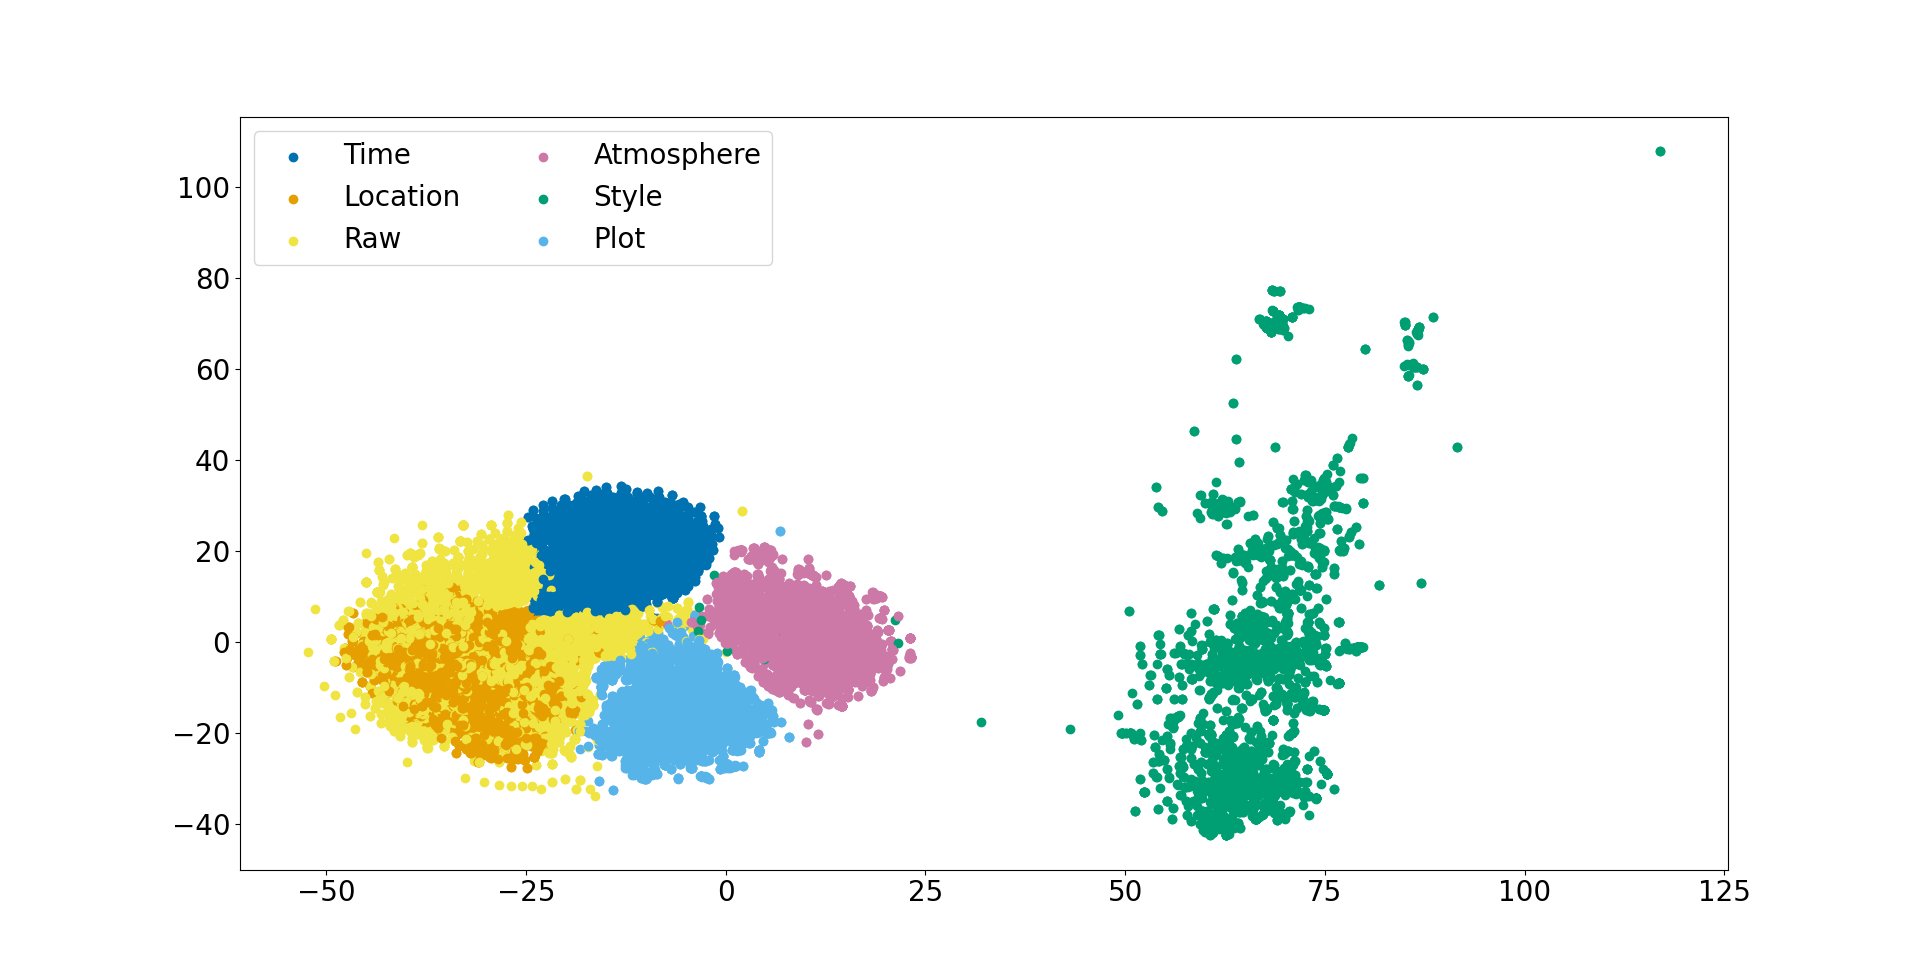
\includegraphics[width=\textwidth,trim={5cm 0 4.4cm 0},clip]{figures/facet_projection_litrec_raw}
		\caption{LitRec dataset}
		\label{fig:tsne_litrec}
	\end{subfigure}

	\begin{subfigure}{\linewidth}
		\centering
		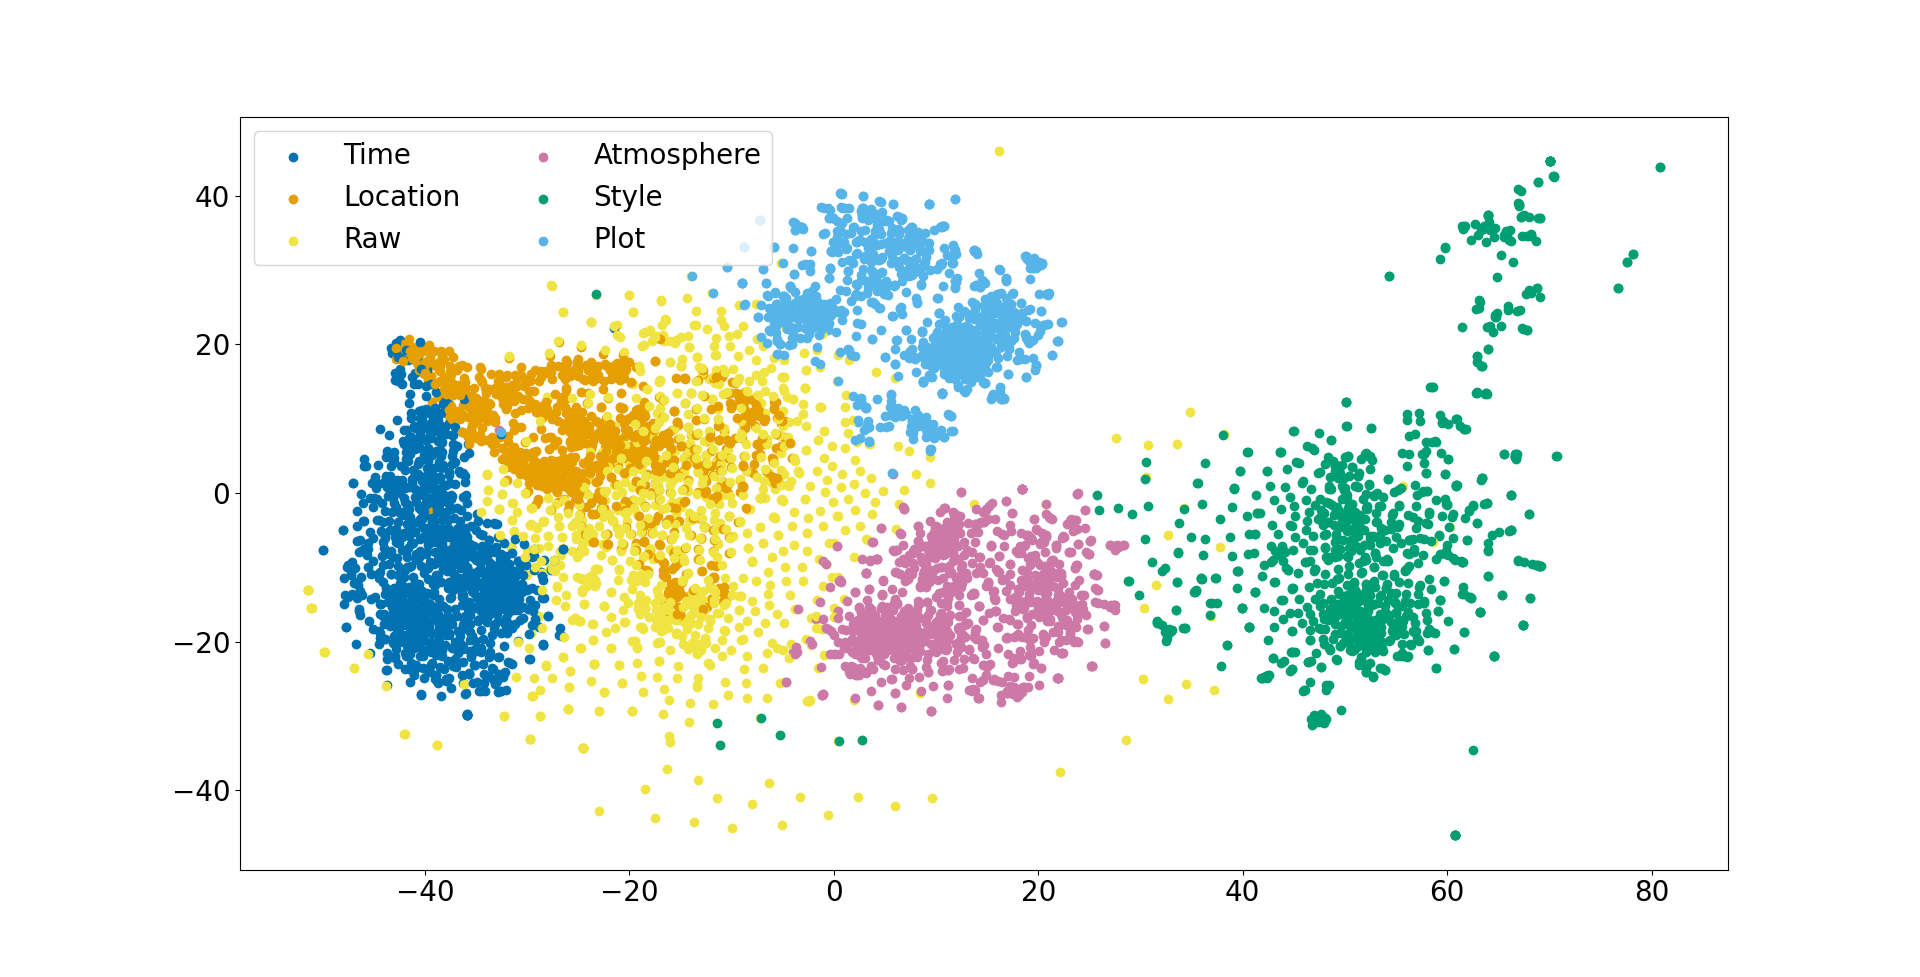
\includegraphics[width=\linewidth,trim={5cm 0 4.4cm 0},clip]{figures/facet_projection_goodreads_raw}
		\caption{MGG dataset}
		\label{fig:tsne_gcc}
	\end{subfigure}
	
	\begin{subfigure}{\linewidth}
		\centering
		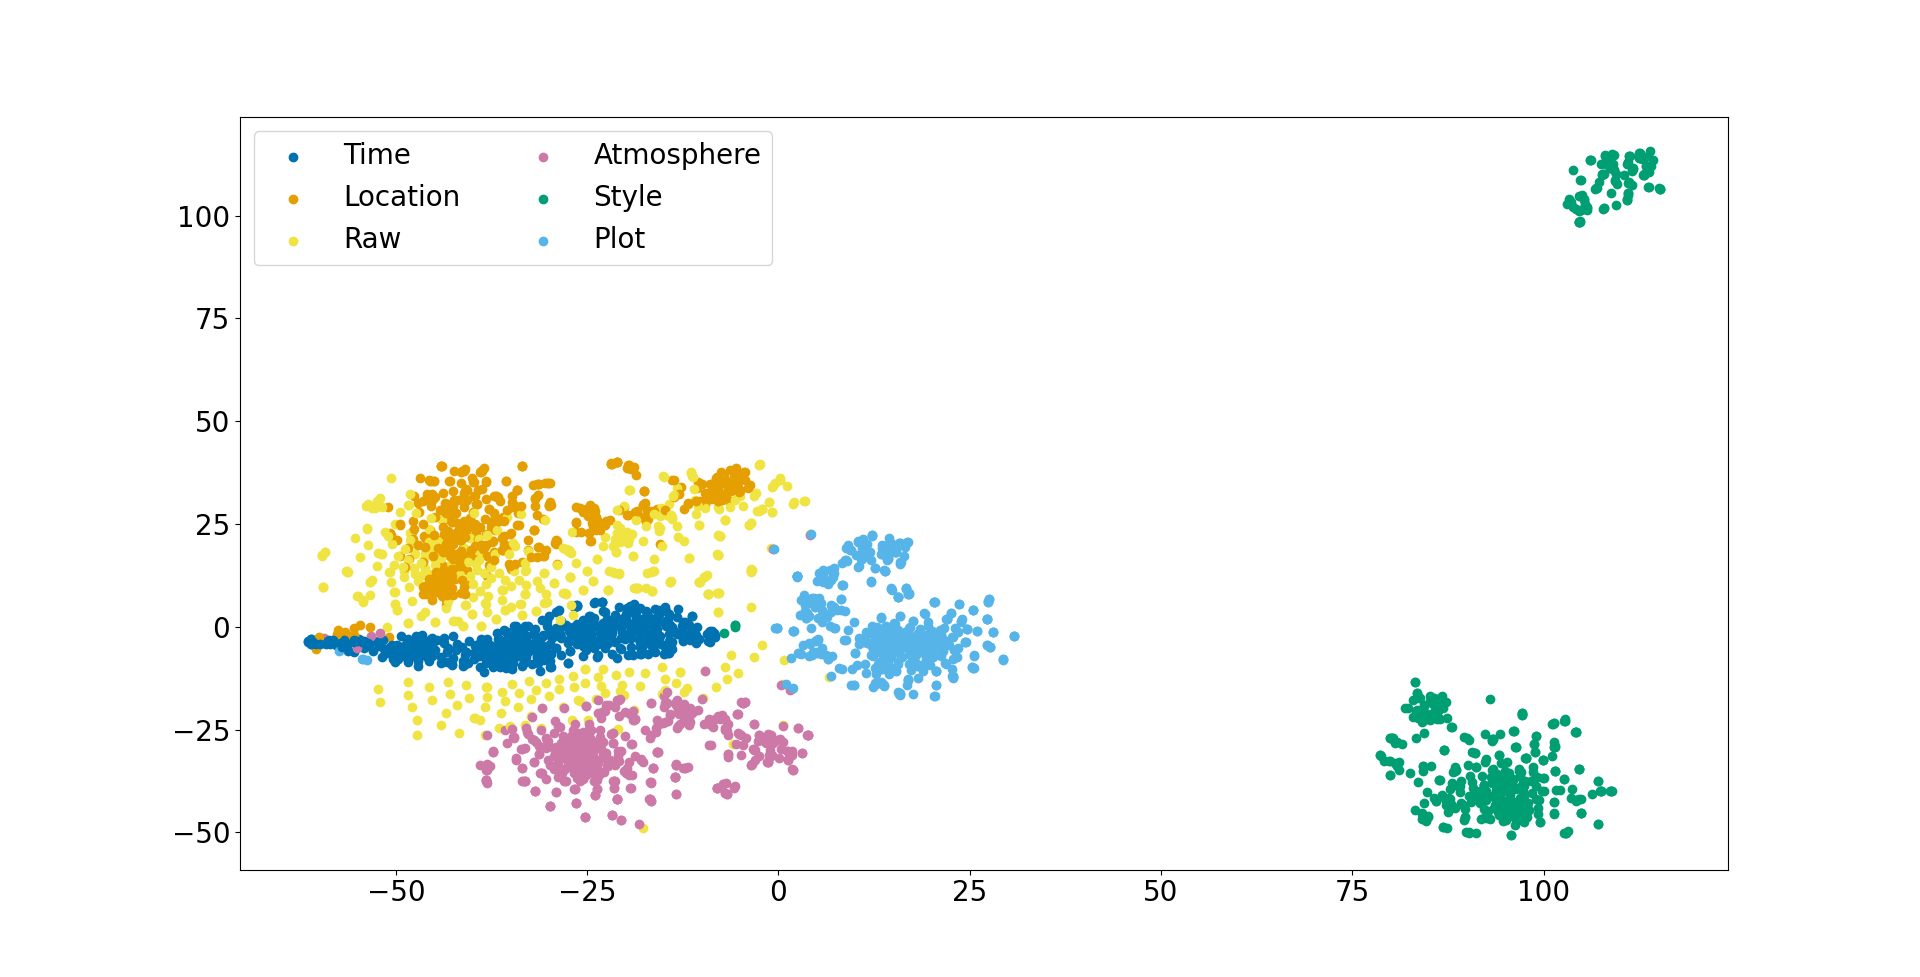
\includegraphics[width=\linewidth,trim={5cm 0 4.4cm 0},clip]{figures/facet_projection_dta_raw}
		\caption{DTA dataset}
		\label{fig:tsne_dta}
	\end{subfigure}
	\caption{t-SNE projection of \emph{lib2vec} facets for different datasets.}
	\label{fig:tsne}
\end{figure}

\section{Similarity Neighborhoods}
% TODO explain/overview
Figure~\ref{fig:neighborhood_overall} and Figure~\ref{fig:neighborhood_content} and Table~\ref{tab:content_qualitative}

\begin{figure*}
	\centering
	\fbox{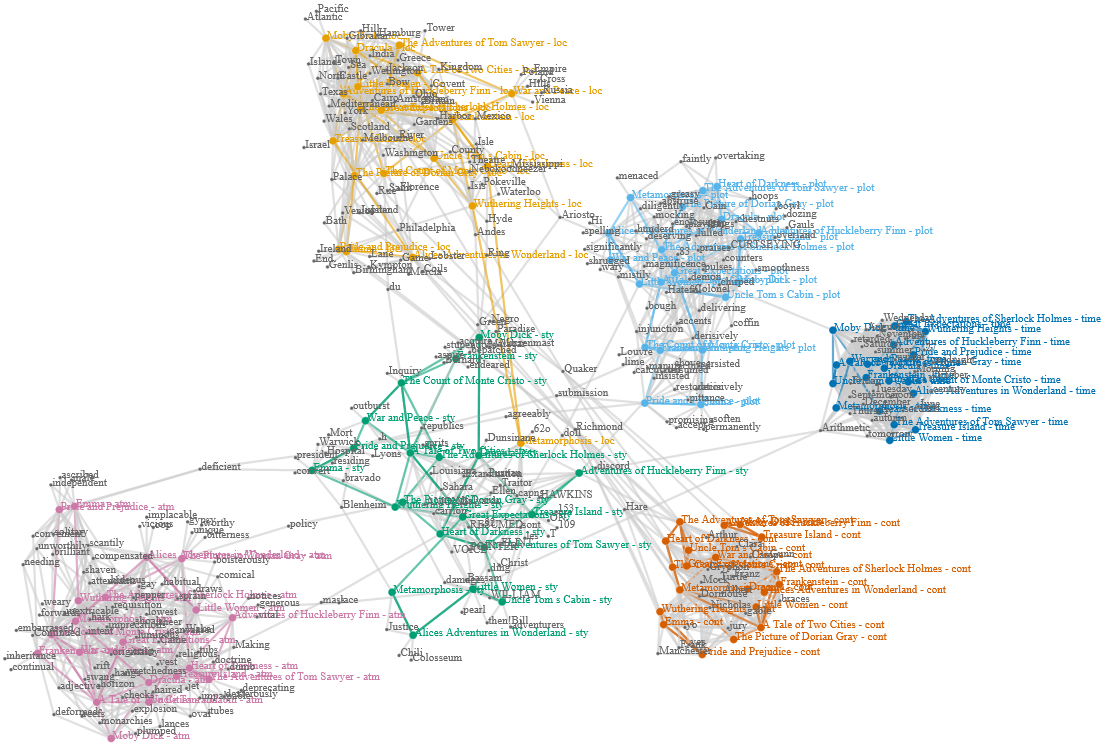
\includegraphics[width=\linewidth]{figures/complete_neighborhood_new}}
	\caption{Neighborhood graph with a force-directed layout for the time (time, dark blue), location (loc, yellow), style (sty, green), atmosphere (atm, pink), plot (bright blue, plot), and content (cont, orange). Links to the first and second document neighbor are displayed for each document. Furthermore, links to the seven most relevant words are added, if they are in the top-\textit{50} neighborhood of a document and within a TF-IDF-rank of 5,000.}
	\label{fig:neighborhood_overall}
\end{figure*}

\begin{figure*}
	\centering
	\fbox{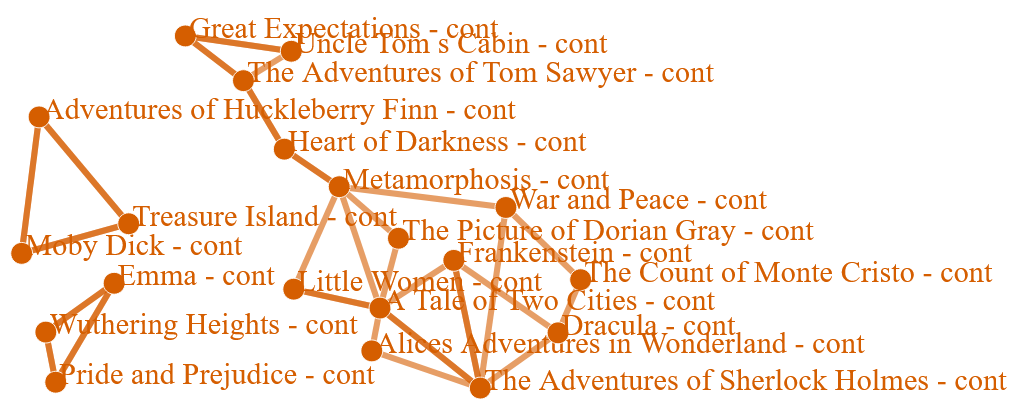
\includegraphics[width=\linewidth]{figures/content_neighborhood_rm2}}
	\caption{Zoomed in neighborhood graph of the content facet for two document neighbors. Links between words and documents are removed.}
	\label{fig:neighborhood_content}
\end{figure*}


\begin{table*}
	\centering
	\footnotesize
	\begin{tabular}{lll}
		\toprule
		Book &                                  First Neighbor &                                 Second Neighbor \\
		\midrule
		%		Adv. of Huckleberry Finn &       Adv. of Tom Sawyer &         Treasure Island \\
		%		Moby Dick &               Heart of Darkness &                            Dracula \\
		%		Pride and Prejudice &                               Emma &                      Frankenstein \\
		%		Adv. of Sherlock Holmes &                       Frankenstein &         Adv. of Tom Sawyer \\
		%		Adv. of Tom Sawyer &         Treasure Island &     Adv. of Huckleberry Finn \\
		%		The Count of Monte Cristo &                     Frankenstein &               Pride and Prejudice \\
		%		The Picture of Dorian Gray &                Wuthering Heights &                 Little Women \\
		%		Treasure Island &       Adv. of Tom Sawyer &               Heart of Darkness \\
		%		Uncle Tom's Cabin & Alice's Adv. in Wonderland &                           Dracula \\
		%		War and Peace &     The Count of Monte Cristo &                     Frankenstein \\
		%		Wuthering Heights &        The Picture of Dorian Gray &                 Little Women \\
		%		Alice's Adv. in Wonderland &        Uncle Tom's Cabin &          A Tale of Two Cities \\
		%		A Tale of Two Cities &            Great Expectations & Alice's Adv. in Wonderland \\
		%		Dracula & Alice's Adv. in Wonderland &        Uncle Tom's Cabin \\
		%		Emma &               Pride and Prejudice &                     Frankenstein \\
		%		Frankenstein &       Adv. of Tom Sawyer &     The Count of Monte Cristo \\
		%		Great Expectations &          A Tale of Two Cities & Alice's Adv. in Wonderland \\
		%		Heart of Darkness &                     Moby Dick &         Treasure Island \\
		%		Little Women &        The Picture of Dorian Gray &                Wuthering Heights \\
		%		Metamorphosis &            Great Expectations &          A Tale of Two Cities \\
		Adv. of Huckleberry Finn &                           \textbf{Moby Dick} &                     \textbf{Treasure Island} \\
		Moby Dick &      \textbf{Adv. of Huckleberry Finn} &                     \textbf{Treasure Island} \\
		Pride and Prejudice &                                \textbf{Emma} &                  \textbf{Wuthering Heights} \\
		The Adv. of Sherlock Holmes &                        \textbf{Frankenstein} &                A Tale of Two Cities \\
		The Adv. of Tom Sawyer &                   Heart of Darkness &                  Great Expectations \\
		The Count of Monte Cristo &                       \textbf{War and Peace} &                             Dracula \\
		The Picture of Dorian Gray &                \textbf{A Tale of Two Cities} &                       \textbf{Metamorphosis} \\
		Treasure Island &      \textbf{Adv. of Huckleberry Finn} &                           \textbf{Moby Dick} \\
		Uncle Tom's Cabin &                  Great Expectations &        \textbf{The Adv. of Tom Sawyer} \\
		War and Peace &                       Metamorphosis &   The Adv. of Sherlock Holmes \\
		Wuthering Heights &                                \textbf{Emma} &                 \textbf{Pride and Prejudice} \\
		Alice's Adv. in Wonderland &   The Adv. of Sherlock Holmes &                A Tale of Two Cities \\
		A Tale of Two Cities &   The Adv. of Sherlock Holmes &                        Little Women \\
		Dracula &   \textbf{The Adv. of Sherlock Holmes} &                        Frankenstein \\
		Emma &                 \textbf{Pride and Prejudice} &                   \textbf{Wuthering Heights} \\
		Frankenstein &   \textbf{The Adv. of Sherlock Holmes} &                A Tale of Two Cities \\
		Great Expectations &                   Uncle Tom's Cabin &        The Adv. of Tom Sawyer \\
		Heart of Darkness &        The Adv. of Tom Sawyer &                       Metamorphosis \\
		Little Women &                A Tale of Two Cities &                       Metamorphosis \\
		Metamorphosis &                   Heart of Darkness &                A Tale of Two Cities \\
		\bottomrule
	\end{tabular}
	\caption[First and Second Neighbors of the Content Facet.]{First and second neighbors of the content facet. Obvious thematic similarities are highlighted in bold.}
	\label{tab:content_qualitative}
\end{table*}

\section{Extended Description of Datasets}

\paragraph{Corpus of German-Language Fiction (CGF).}
The Corpus of German Fiction by~\citet{fischer_corpus_2017} consists of 3,219 prose books.
It contains two sub-corpora, one for 484 works of 18 English, Russian, and French authors and one for 2,735 works by 549 German authors.
The only metadata available is information about the author, title, and year.
Most of the texts are written in the time range between 1840-1930.
As shown in Table~\ref{tab:datasets_overview} it is one of the largest corpora in terms of sentence numbers, token lengths, and vocabulary sizes.

\paragraph{Series CGF (S-CGF).}
This sub-corpus of the CGF dataset is specially composed for this work and contains series of books.
To select books that belong to the same book series, the indicator words of the title are used, such as \textit{Band}, (\textit{volume}) or \textit{Teil} (\textit{Part}).
In most cases, books in the same series have the same title but a specific series number.
All books of one specific author are compared by title matching for identification.
In terms of total length, the S-CGF is roughly ten times smaller than the original corpus according to Table~\ref{tab:datasets_overview}.
However, the mean and median lengths are higher, which implies that books belonging to a series have more tokens, more words in the vocabulary, and more sentences, compared to non-series books.

\paragraph{Deutsches Text Archiv (DTA).}
The DTA corpus contains 4,422 German texts of different domains including 765 works of belles lettres for the time range between the 16th and 20th century~\citep{berlin-brandenburgischen_akademie_der_wissenschaften_deutsches_2021}.
Since the German language has changed significantly in the past 400 years, texts published before 1800 have been excluded, leaving 459 texts.
The period starting in 1800 also coincides more with the CGF and BoCo eras.
Other genres in the corpus such as news or scientific articles are dismissed since they are not relevant for the present work.
The books in the corpus are usually annotated with title, author, and year information, however, some works are of unknown authors.
The corpus also contains information about book series in the titles of 176 books.
Therefore, series books can be identified by indicator words such as \textit{Band} similar to CGF and S-CGF.

\paragraph{LitRec.}
LitRec is a dataset that contains full-texts of English books from Project Gutenberg.
The 3,458 full-texts written by 1,109 authors are tokenized and annotated with POS-tags by~\citet{vaz_litrec_2012}.
However, only 3,075 books remain after the removal of corrupted files.
Nevertheless, LitRec is the largest English-language book corpus available.
It is often used in recommendation research contexts because it contains 35,507 ratings of book readers.

\paragraph{Gutenberg and Genres (MGG).}
This corpus by~\citet{maharjan_multi-task_2017} contains 1,003 full-texts of English books and was built to evaluate book models within success and genre prediction tasks. 
For this reason, it contains genre information and a binary label of success for each book.
Success is measured by Goodreads ratings. 
If a book has an average rating higher than $3.5$ stars from ten or more people, it is considered successful.

\paragraph{Book Comparison (BoCo).}
This corpus consists of 20 popular English books from Project Gutenberg.\footnote{\url{https://www.gutenberg.org/} (visited on 01/04/2021.)}
These 20 books were selected in terms of popularity measured by the top-\textit{100} download numbers within December 2020.
For legal reasons, we cannot share the full-texts. 
However, these texts can be accessed in the English version of Project Gutenberg. 
Though, only 68 participants have rated the similarity for book triplets, since the remaining 13 participants did not know any book of the overall selected triplets.
BoCo contains human assessments about the similarity of triplets for certain facets.
These facets are time, location, atmosphere, content, and plot. 
Assessments of style are not collected, since the question of style similarity can only be answered with detailed knowledge of the text.
Such detailed knowledge is considered an excessive requirement for participation in the study.
Besides, BoCo contains assessments of the overall similarity.

%\begin{table*}
%	\centering
%	\footnotesize
%	\begin{tabular}{lllllll}
%		\toprule
%		{} &  CGF &  S-CGF &       DTA &     LitRec &  MGG &  BoCo \\
%		\midrule
%		Amount of Books      &         3.22K &            208 &      459 &     3.08K &                1K &                 20 \\
%		Language          &           GER &            GER &      GER &        EN &                EN &                 EN \\
%		\midrule
%		Tokens Sum      &          204M &          22.2M &    25.6M &      275M &             16.7M &              3.76M \\
%		Tokens Median     &         45.8K &          81.4K &    43.9K &     72.7K &             16.9K &               145K \\
%		Tokens IQR        &         75.4K &            67K &    55.1K  &    80.6K &             10.9K &               138K \\
%		Tokens Min        &            78 &          3.02K &      260 &     2.66K &               720 &                25K \\
%		Tokens Max        &         1.03M &           309K &     245K &      673K &             61.6K &               672K \\
%		\midrule
%		Vocabulary Sum  &         26.3M &          2.63M &    3.84M &     22.3M &             2.87M &               198K \\
%		Vocabulary Median &         7.24K &          11.1K &    7.46K &     6.97K &             2.83K &              8.85K \\
%		Vocabulary IQR    &         8.49K &          5.59K &    6.58K &     4.34K &             1.48K &               5.1K \\
%		Vocabulary Min    &            64 &          1.09K &      125 &       903 &               335 &              2.71K \\
%		Vocabulary Max    &         53.4K &          37.1K &    28.2K &     53.2K &             9.62K &              19.4K \\
%		\midrule
%		Author Mean       &          5.68 &           4.24 &     2.07 &      2.77 &              2.13 &               1.18 \\
%		Author STD        &          8.53 &           4.20 &     2.29 &      6.25 &              2.42 &               0.38 \\
%		Author [Min, Max] &       [1, 78] &        [2, 21] &  [1, 19] &  [1, 150] &           [1, 24] &             [1, 2] \\
%		\midrule
%		Series Mean       &          2.53 &           2.53 &     3.20 &         - &                 - &                  - \\
%		Series STD        &          1.13 &           1.13 &     1.99 &          - &                 - &                  - \\
%		Series [Min, Max] &        [2, 8] &         [2, 8] &  [2, 14] &         - &                 - &                  - \\
%		\midrule
%		Genre Mean        &             - &              - &        - &         - &            125.38 &                  - \\
%		Genre STD         &             - &              - &        - &         - &             58.59 &                  - \\
%		Genre [Min, Max]  &             - &              - &        - &        - &         [80, 258] &                  - \\
%		\bottomrule
%	\end{tabular}
%	\caption[Overview of Different Dataset Characteristics]{Overview of dataset characteristics.
%		In addition to the number of books for each corpus and language, values for token counts and vocabulary sizes are reported.
%		For tokens and vocabulary words, the values include the total numbers, the median, the interquartile distance ratio (IQR), as well as the minimum and maximum for each document.
%		Besides, the mean, the standard deviation (STD), minima, and maxima are reported for authors, series, and genres.
%		For example, these values show how many books belong to an author on average.}
%	\label{tab:datasets_overview}
%\end{table*}

\section{Influence of Different Text Lengths on Similarity}
\label{sec:long_text_problem}
Working with the full-text of books opens up special challenges, for example longer texts may have an impact on the representation of a book.
Length is a simple criterion to discriminate and could therefore implicitly learned by an embedding model.
As a consequence, the embedding may be biased by length.
To counteract this length bias, the relationship between cosine similarity and difference in book length is investigated in this section.

Length similarity is defined as $min(a,b) / max(a, b)$ where $a, b$ are the given token numbers of two documents for this work.
The resulting value lies in the interval of $[0, 1]$.
The higher the length similarity value is, the more similar two document lengths are.

\begin{figure}
	\centering
	\includegraphics[width=\linewidth]{figures/length_influence_book2vec_german_books}
	\caption{Opposed cosine similarity and length similarity for the \emph{lib2vec} algorithm.
		The color indicates the number of tokens for the first document which is compared with a second one.
		The histograms on the axis show the frequencies of similarity values. 
		The regression lines are plotted based on a subset of different defined text lengths.}
	\label{fig:length_influence_b2v}
\end{figure}

Figure~\ref{fig:length_influence_b2v} shows a scatter plot for the cosine and length similarity.
Additionally, on each similarity axis, a histogram depicts the total number of elements according to similarity.
Regression lines are plotted for a better understanding of the correlation between both.
The dataset is split by length into three similar-sized parts, representing small documents, medium-sized documents, and large documents.
Small documents have token numbers smaller than the 0.33 quantile of the overall corpus, large documents are larger than the 0.66 quantile, medium-sized documents are in the range between the 0.33 and the 0.66 quantiles.
A regression line with a higher positive or negative slope indicates a higher positive or negative correlation.
The correlation between text length and cosine similarity for small and medium texts is very similar because the regression lines are almost parallel.
Very large documents have a higher slope.
The larger slope for long documents implies that long documents are more likely to receive a higher cosine similarity if the documents are similar in length.
The horizontal histogram in Figure~\ref{fig:length_influence_b2v} shows that the cosine similarity is normally distributed over all documents.
However, the vertical histogram for length similarity shows that most documents are very different in size as it is skewed to the lower end of the axis indicating length similarity.
It also becomes clear that the length similarity is not normally distributed.
As a result, most documents with a cosine similarity around 0.5 are very dissimilar in length.

\begin{table*}[ht]
	\centering
%	\footnotesize
	\begin{tabular}{lrrrr}
		\toprule
		Algorithm & Total [p] & Short [p] & Medium [p] & Long [p] \\
		\midrule
		AVG W2V &   0.20 [0.00] &    0.09 [0.00] &     0.15 [0.00] &   0.23 [0.00] \\
		doc2vec &  -0.16 [0.00] &   -0.06 [0.00] &    -0.14 [0.00] &  -0.15 [0.00] \\
		\emph{lib2vec} &   0.04 [0.00] &    0.03 [0.00] &     0.03 [0.00] &   0.07 [0.00] \\
		\bottomrule
	\end{tabular}
	\caption[Spearman Correlation between Length and Cosine Similarity]{Spearman correlation and p-values between length and cosine similarity for length-specific sub-datasets for different embedding algorithms.}
	\label{tab:text_length_correlation}
\end{table*}

\begin{table*}[ht!]
	\centering
	\footnotesize
	\begin{tabular}{L{0.3cm}lrrrrrrrr}
		\toprule
		& Dataset &     DTA &  DTA-L &  DTA-M &  DTA-Sh &  CGF &  CGF-L &  CGF-M &  CGF-Sh \\
		Task & Algorithm &         &            &             &            &               &                     &                      &                      \\
		\midrule
		A 	& BoW &  0.6913 &     0.8145 &      0.7772 &     0.6811 &        0.6687 &              0.6912 &               0.6117 &              0.5732 \\
		& AVG W2V &  0.6730 &     0.8140 &      0.6834 &     0.7380 &        0.6498 &              0.6432 &               0.5674 &              0.5766 \\
		& doc2vec &  0.7442 &     0.8860 &      0.7803 &     0.7910 &        0.7530 &              0.7417 &               0.7253 &              0.6980 \\
		& BERT &  0.3956 &     0.4157 &      0.2954 &     0.3929 &        0.6015 &              0.5063 &               0.5144 &              0.5931 \\
		& RoBERTa &  0.3809 &     0.3704 &      0.2989 &     0.3871 &        0.5466 &              0.4268 &               0.4433 &              0.5008 \\
		& XLM &  0.3769 &     0.3742 &      0.3081 &     0.3829 &        0.5821 &              0.4817 &               0.4881 &              0.5278 \\
		& P-SIF &  0.6642 &     0.7685 &      0.7264 &     0.6286 &        0.6796 &              0.6882 &               0.6092 &              0.6055 \\
%		\midrule
%		A & lib2vec SUM &  0.7913 &     0.9183 &      0.8061 &     0.8443 &        0.8387 &              0.8983 &               0.8545 &              0.7614 \\
%		& lib2vec AVG &  0.7867 &     0.9109 &      0.8146 &     0.8459 &        0.8190 &              0.8765 &               0.8290 &              0.7276 \\
%		& lib2vec CON &  0.8012 &     0.9198 &      0.8502 &     0.8493 &        0.8733 &              0.9352 &               0.8854 &              0.8065 \\
%		& lib2vec PCA &  0.7962 &     \textbf{0.9275} &      0.8499 &     0.8149 &        0.8625 &              0.9386 &               0.8960 &              0.7823 \\
		& \emph{lib2vec} AUTO &  \textbf{0.8014} &     \textbf{0.9228} &      \textbf{0.8642} &     \textbf{0.8621} &        \textbf{0.8599} &              \textbf{0.9287} &               \textbf{0.8790} &              \textbf{0.7946} \\
%		& lib2vec DBOW CON &  0.7987 &     0.9134 &      0.8357 &     0.8377 &        0.8864 &              0.9533 &               0.9082 &              \textbf{0.8087} \\
%		& lib2vec DBOW PCA &  0.7932 &     0.9245 &      0.8499 &     0.7830 &        \textbf{0.8924} &              \textbf{0.9550} &              \textbf{ 0.9234} &              0.7940 \\
		\midrule
		S 	& BoW &  0.9204 &     0.8614 &      0.8297 &     \textbf{0.9025} &        0.8005 &              0.7358 &               0.7964 &              0.\textbf{4397} \\
		& AVG W2V &  0.8909 &     0.8646 &      0.7640 &     \textbf{0.9025} &        0.6409 &              0.6573 &               0.6325 &              0.3712 \\
		& doc2vec &  0.9367 &     0.8823 &      0.8321 &     \textbf{0.9025} &        0.7710 &              0.7591 &               0.7641 &              0.\textbf{4397} \\
		& BERT &  0.3877 &     0.4210 &      0.2904 &     0.4464 &        0.6410 &              0.6600 &               0.5809 &              0.4302 \\
		& RoBERTa &  0.3392 &     0.3629 &      0.2878 &     0.4470 &        0.3989 &              0.4145 &               0.3843 &              0.3151 \\
		& XLM &  0.3555 &     0.3748 &      0.3026 &     0.4476 &        0.5406 &              0.5625 &               0.4730 &              0.3151 \\
		& P-SIF &  0.8871 &     0.8574 &      0.7944 &     0.8455 &        0.6961 &              0.6891 &               0.6879 &              0.3696 \\
%		\midrule
%		S & lib2vec SUM &  0.9600 &     0.9095 &      0.8375 &     \textbf{0.9025} &        0.8659 &              0.8185 &               0.7954 &              0.2996 \\
%		& lib2vec AVG &  0.9548 &     0.9051 &      0.8375 &     \textbf{0.9025} &        0.8617 &              0.8175 &               0.7954 &              0.2996 \\
		& \emph{lib2vec} CON &  \textbf{0.9730} &     \textbf{0.9144} &      \textbf{0.8552} &     \textbf{0.9025} &        \textbf{0.8905} &              \textbf{0.8383} &               \textbf{0.8133} &              0.3346 \\
%		& lib2vec PCA &  \textbf{0.9752} &     0.9183 &      0.8512 &     \textbf{0.9025} &        0.8706 &              0.8363 &               0.7938 &              0.2996 \\
%		& lib2vec AUTO &  0.9740 &     0.9116 &      \textbf{0.8612} &     \textbf{0.9025} &        0.8584 &              0.8203 &               0.7880 &              0.3346 \\
%		& lib2vec DBOW CON &  0.9666 &     0.9155 &      0.8576 &     \textbf{0.9025} &        0.8656 &              0.8186 &               0.8012 &              0.3696 \\
%		& lib2vec DBOW PCA &  0.9630 &     \textbf{0.9195} &      0.8576 &     0.8455 &        0.8465 &              0.7996 &               \textbf{0.8133} &              \textbf{0.4047} \\
		\bottomrule
	\end{tabular}
	\caption[Author and Series Task Results of Baselines and \emph{lib2vec} Variants]{Author (A) and Series (S) Task NDCG scores of baseline and different combination variants of \emph{lib2vec} with strict specific word filter on different corpora and short (Sh), medium (M) and large (L) length specific sub-corpora. The highest values for each task and dataset are highlighted in bold.}
	\label{table:ndcg_multi}
\end{table*}

\renewcommand{\tabcolsep}{2.5pt}
\begin{table}[ht!]
	\centering
	\footnotesize
	\begin{tabular}{@{}L{0.5cm}lrrrrr@{}}
		\toprule
		& Dataset               & MGG             & MGG-L           & MGG-M           & MGG-Sh          \\
		Task & Algorithm             &                 &                 &                 &                 \\ \midrule
		A    & BoW                   & 0.5294          & 0.5702          & 0.5507          & 0.4645          \\
		& AVG W2V               & 0.5129          & 0.5644          & 0.5178          & 0.4579          \\
		& doc2vec               & 0.6893 & 0.7727 & 0.7555 & 0.5821 \\
		& P-SIF                 & 0.5530          & 0.6349          & 0.5613          & 0.4463          \\
		& BERT                  & 0.4251          & 0.4279          & 0.4253          & 0.3403          \\
		& RoBERTa               & 0.4168          & 0.4192          & 0.4278          & 0.3364          \\
		& XLM                   & 0.4214          & 0.4273          & 0.4348          & 0.3579          \\ 
%		\midrule
%		A    & lib2vec SUM      & 0.7087          & 0.7949          & 0.7948          & 0.5910          \\
%		& lib2vec AUTO     & 0.6611          & 0.7204          & 0.7053          & 0.5665          \\
%		& lib2vec AVG      & 0.7124          & 0.8089          & 0.7908          & 0.5818          \\
%		& lib2vec CON      & 0.6660          & 0.7182          & 0.7080          & 0.5740          \\
%		& lib2vec PCA      & 0.6712          & 0.7341          & 0.7269          & 0.5685          \\
%		& lib2vec DBOW CON & 0.7614          & 0.8308          & 0.8491          & 0.6025          \\
		& \emph{lib2vec} PCA & \textbf{0.7819} & \textbf{0.8605} & \textbf{0.8761} & \textbf{0.6218} \\ \midrule
		G    & BoW                   & 0.9880          & 0.8317          & 0.8201          & 0.9329          \\
		& AVG W2V               & 0.9881          & 0.8354          & 0.8260          & \textbf{0.9351} \\
		& doc2vec               & 0.9884 & 0.8410 & 0.8284          & 0.9262          \\
		& P-SIF                 & 0.9878          & 0.8439          & 0.8333 & 0.9319          \\
		& BERT                  & 0.9876          & 0.8189          & 0.8112          & 0.9265          \\
		& RoBERTa               & 0.9868          & 0.8170          & 0.8073          & 0.9255          \\
		& XLM                   & 0.9874          & 0.8193          & 0.8134          & 0.9260          \\ 
%		\midrule
%		G    & lib2vec SUM      & 0.9887          & 0.8533          & 0.8429          & 0.9310          \\
%		& lib2vec AUTO     & 0.9893          & 0.8654          & 0.8584          & 0.9404          \\
%		& lib2vec AVG      & 0.9885          & 0.8456          & 0.8322          & 0.9283          \\
		& \emph{lib2vec} CON      & \textbf{0.9898} & \textbf{0.8681}          & \textbf{0.8679} & \textbf{0.9468} \\
%		& lib2vec PCA      & 0.9892          & \textbf{0.8683} & 0.8669          & 0.9433          \\
%		& lib2vec DBOW CON & 0.9883          & 0.8408          & 0.8206          & 0.9294          \\
%		& lib2vec DBOW PCA & 0.9882          & 0.8427          & 0.8324          & 0.9296          \\ \bottomrule
	\end{tabular}
	\caption[]{Author (A) and Genre (G) Task NDCG scores for baseline and different combination variants of \emph{lib2vec} with strict specific word filter on MGG. The highest values for each task are highlighted in bold.}
	\label{table:ndcg_gcc}
\end{table}

For an overview of other basic algorithms such as averaged word embeddings or doc2vec, the correlation coefficients are computed and shown in Table~\ref{tab:text_length_correlation}.
Pearson's correlation is not well-suited for analysis because the length similarity is not normally distributed.
Instead, Spearman's correlation is considered.
The null hypothesis $H_0$ of this Spearman correlation test states there is no correlation between cosine and length similarity.
The opposing hypothesis, $H_1$, assumes a correlation.

A value close to $0$ for the Spearman coefficient indicates a small correlation.
According to Table~\ref{tab:text_length_correlation}, the cosine similarity values for \emph{lib2vec} are less correlated with the cosine similarity compared with other alternatives for all sub-datasets and the complete dataset.
For the sub-dataset created from large documents, the strength of the correlation is higher than in sub-datasets created from smaller documents.
The slope of the regression line in Figure~\ref{fig:length_influence_b2v} matches the correlation coefficients in Table~\ref{tab:text_length_correlation} of \emph{lib2vec} roughly.
This means, the longer the documents are, the more correlated is cosine similarity with length similarity.
Nevertheless, the p-value for all approaches is very small, which implies that $H_0$ has to be rejected in every case.
In summary, a correlation between length and similarity is measured in all approaches, which means all approaches are affected by this length bias.
However, their higher correlation values imply that doc2vec and word2vec are more biased by length than \emph{lib2vec}.

\section{Removing Similarity Bias}
\begin{figure*}
	\centering
	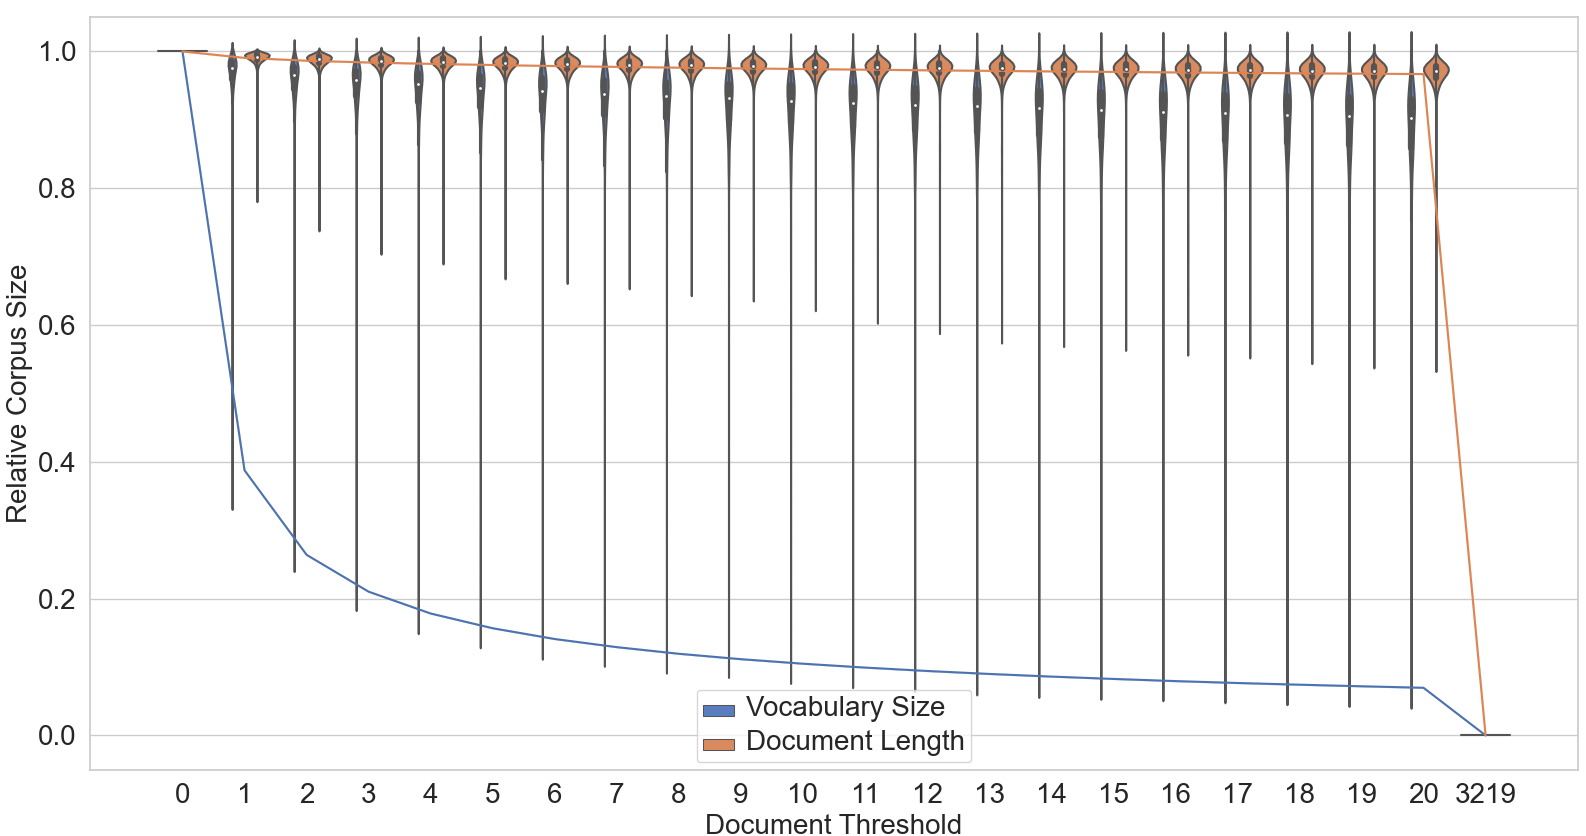
\includegraphics[width=\linewidth]{figures/specific_words_graph}
	\caption{Influence of filtered words on corpus and document sizes for the CGF dataset.
		The filtered words are derived from the document threshold. 
		All words that occur in a less or equal number of documents than this threshold are removed.
		The violin plots show the distribution of the loss of all documents for vocabulary size and document length.
		The lines indicate the vocabulary size of the total corpus and the total number of tokens.}
	\label{fig:specific_words}
\end{figure*}
In addition to the problem of similarity predictions being affected by similar text lengths, there may also be a bias for similar texts.
The similarity bias arises from the fact that books of the same series are likely to have very specific words that only occur in one book series.
This makes it theoretically trivial to identify books of the same series if series-specific words are found.
To make sure that the results are not based only on these very specific words, these words are removed from the data.
Since not only books of the same series could be affected, but also for example authors could use very specific own word creations repeatedly, the problem is generalized and considered in terms of the document frequency.
The document frequency of a word or term indicates in how many documents the word or term occurs.
If a term occurs only in a very small number of documents, it is considered very specific in this context.

Figure~\ref{fig:specific_words} shows the influence of the removal of words with a specific document frequency on vocabulary and document sizes.
Removing all words which are occurring only in one document already reduces the vocabulary of the overall corpus by 60\%.
Nevertheless, according to Figure~\ref{fig:specific_words} the total number of tokens is not affected in similar sizes by this reduction.
Furthermore, the influence on document length and vocabulary size is for most documents small, which is shown by the high average values of the violin plots.

To reduce the specific words by document frequency, a threshold value must be set.
Since Figure~\ref{fig:specific_words} does not show discontinuities for document and vocabulary sizes after a certain threshold, the corpus-dependent maximum of series and author books is set as document frequency threshold.
The maximum ensures that all words that occur only by a particular author or in a particular series are excluded.
The filtering by the maximum is referred to as \textit{strict specific word reduction}.
For smaller corpora, the threshold value is set to at least $3$.
\textit{Moderate specific word reduction} is defined as the median. 
The threshold value is set to at least $2$ for \textit{moderate specific word reduction} for smaller corpora.
However, during the first experiments, it turned out that the models perform only slightly worse with \textit{strict specific word reduction} than with \textit{moderate specific word reduction}, which is the reason to focus on \textit{strict specific word reduction}.

\section{Hyperparameters}
\begin{figure}
	\centering
	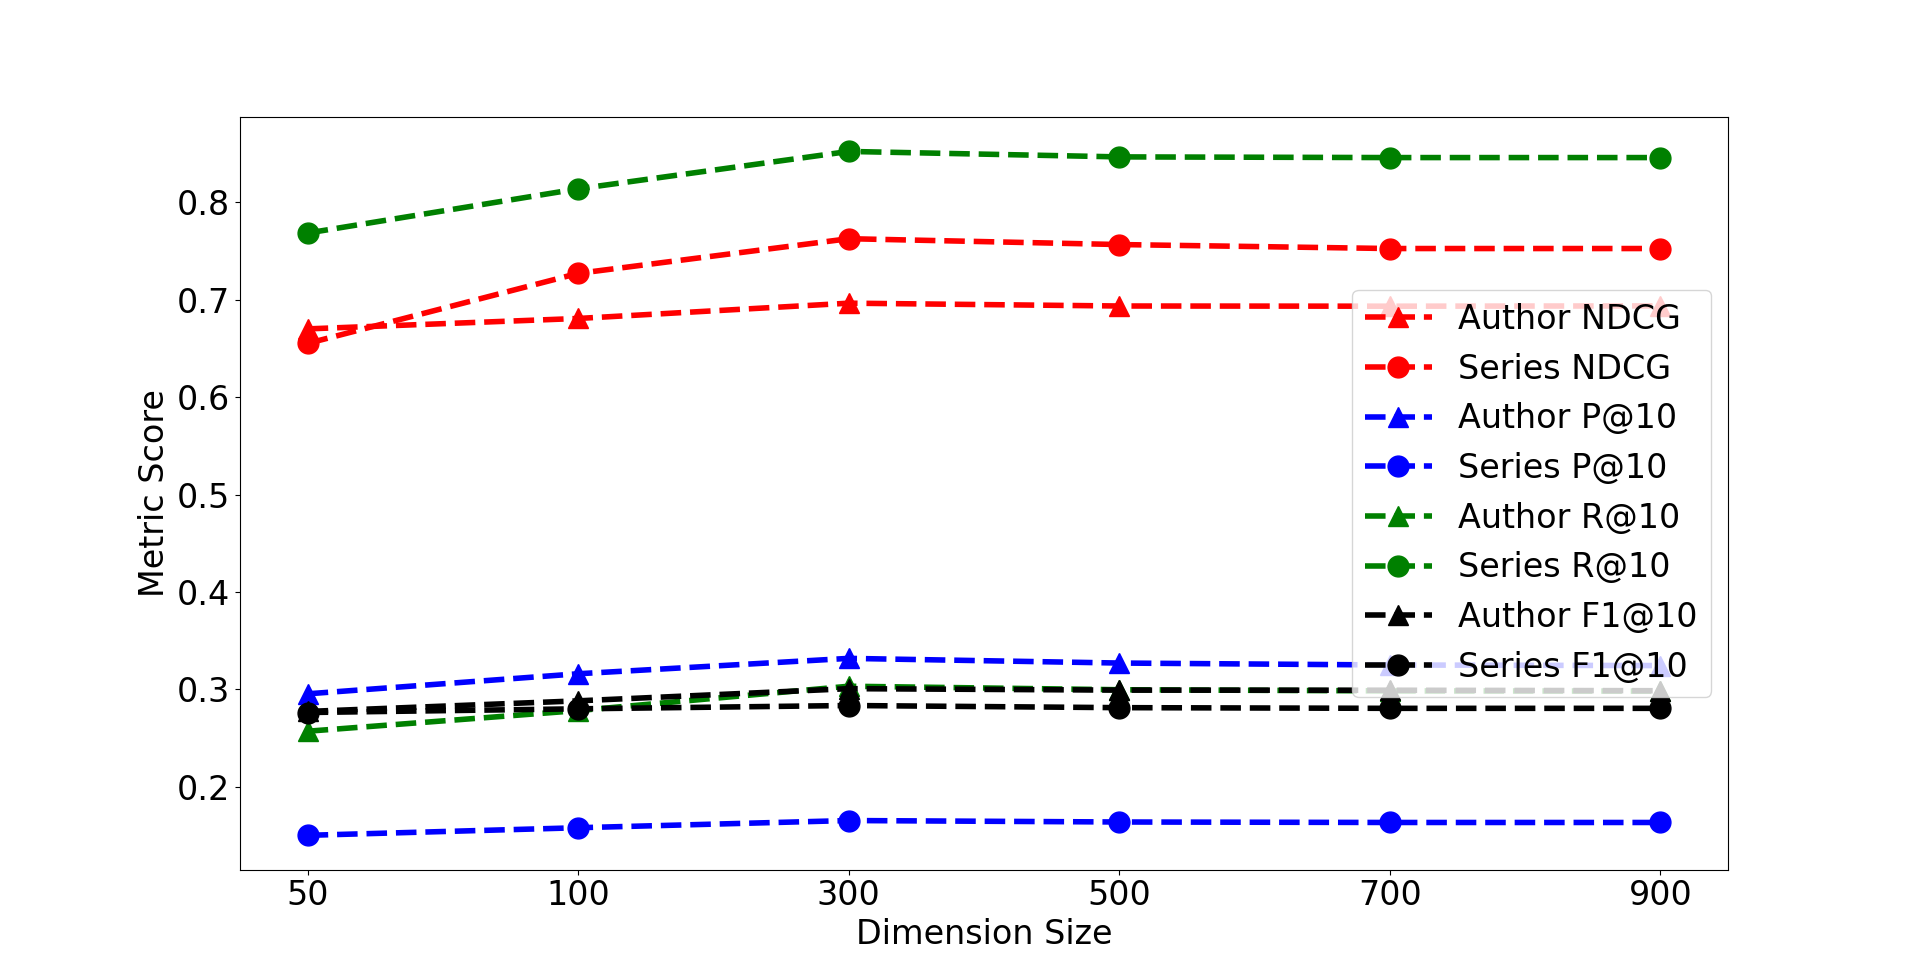
\includegraphics[width=\linewidth]{figures/dimension_performance}
	\caption{doc2vec performance of finding books by the same author or book series in the top-\textit{100} neighborhood.
		The performance of doc2vec is measured in NDCG, precision, recall, and F1 scores for dimension values of  $50, 100, 300, 500, 700, 900$ with a fixed window of $10$ on the CGF dataset.}
	\label{fig:dimension_performance}
\end{figure}

\begin{figure}
	\centering
	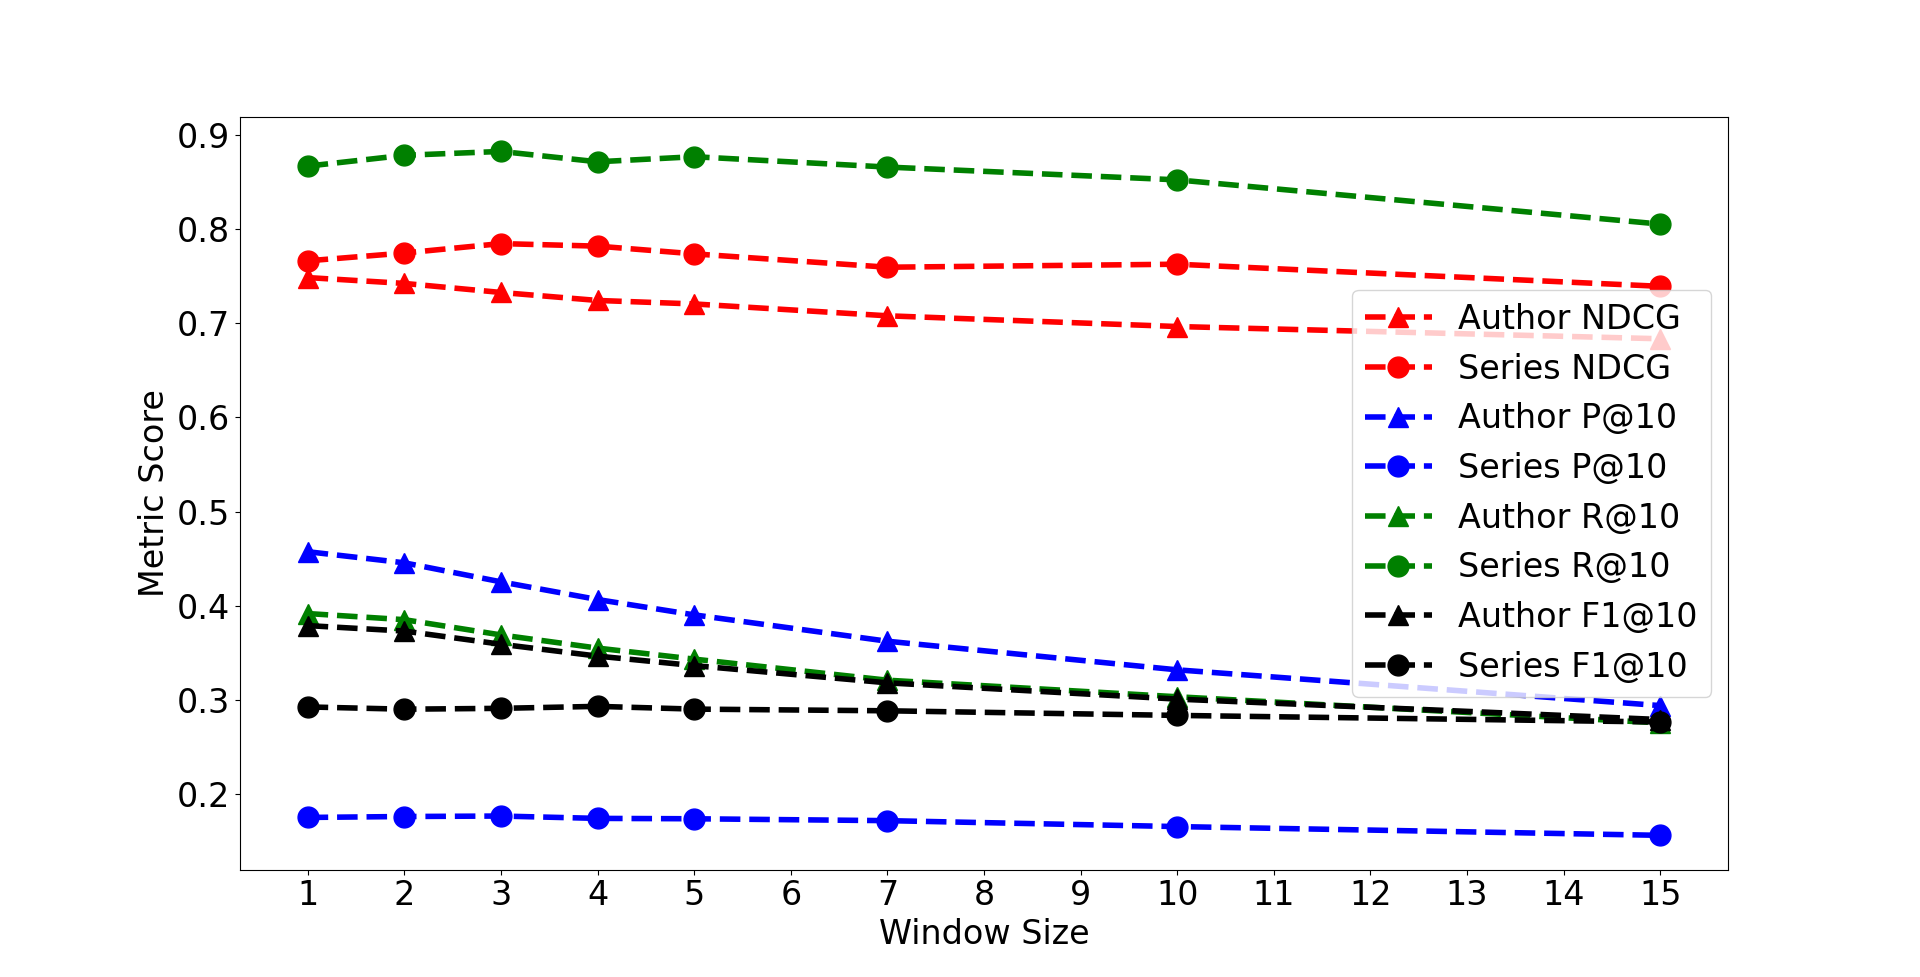
\includegraphics[width=\linewidth]{figures/doc_window_performance}
	\caption{doc2vec performance of finding  books by the same author or book series in the top-\textit{100} neighborhood.
		The performance of doc2vec is measured in NDCG, precision, recall, and F1 scores for window sizes of $1, 2, 3, 4, 5, 7, 10, 15$ with a fixed dimension size of $300$ on the CGF dataset.}
	\label{fig:doc_window_performance}
\end{figure}
The \emph{lib2vec} embeddings are trained using the Gensim~\citep{rehurek_lrec} implementation of doc2vec.
The following hyperparameters are chosen for the trained embeddings by manual tuning:
An embedding dimension of $300$ is considered because this is a common choice for word and document embeddings~\citep{rettig_fusing_2019}.
Besides, experiments are performed with different dimension sizes for doc2vec on the CGF dataset in Figure~\ref{fig:dimension_performance}.
The results confirm, that a dimension size of $300$ is the smallest but best performing choice for different metrics such as NDCG, precision, recall, and F1 in author and series similarity tasks.
A similar experiment is performed to obtain a good choice for the window size in Figure~\ref{fig:doc_window_performance}.
In contrast to dimension size, the window size is the only parameter that is not fixed.
Windows that have a size greater than $5$ perform worse than smaller values.
A window of $5$ is used because this is the value for which \emph{lib2vec} performs best and which is suggested by~\citet{grayson_novel2vec_2016} for semantic relationships.
However, Figure~\ref{fig:doc_window_performance} shows that a window of $5$ is not the best option for doc2vec.
In the case of do2vec, smaller window sizes have a slightly higher score for most metrics.


Each model is trained for $20$ epochs.
The DM option of doc2vec is used as the default variant since DBOW ignores the order of words.
To reduce the configurable parameters, the minimal counter for words is set to $0$, which means no words are excluded by their frequency.
To ensure consistent results, the Python hash seed environment parameter was set to $10$ and all other non-deterministic implementation options are disabled.
The number of workers for the doc2vec embedding algorithm is set to $1$, the seed of the model is set to 42.
The default values are preserved for the other options.
No pre-trained models or further hyperparameter optimization are involved to make results comparable.
The default embeddings of \emph{lib2vec} truncate pseudo-documents that exceed a limit of \numprint{10000} tokens and do not consider a facet window around identified facet words.
All experiments were executed on a Windows midrange machine with 16GB RAM and 48GB swap partition, an AMD Ryzen 5 3600 CPU with 12 cores, and no GPU.
More complex experiments were executed on a Dell PowerEdge R810 server.

\begin{table}[]
	\begin{tabular}{@{}lrr@{}}
		\toprule
		& Parameters & With \emph{lib2vec} \\ \midrule
		BoW 30K         & \numprint{3000}
		 M        & \numprint{3005} M                                     \\
		AVG W2V     & 30 M       & 35 M                                   \\
		doc2vec DM   & 30 M       & 35 M                                   \\
		doc2vec DBOW & 0.1 M      & 0.5 M                                  \\
		BERT         & *110 M      & *110 M                                  \\
		RoBERTa      & *125 M      & *125 M                                  \\
		XLM          & *110 M      & *110 M                                  \\
		P-SIF        & 30 M       & 35 M                                   \\ \bottomrule
	\end{tabular}
	\caption[]{Number of parameters for each model architecture on a corpus of \numprint{3000} novels and a vocabulary of \numprint{100000} words. *values taken from the description of the Hugging Face transformer library.}
\label{tab:parameters}
\end{table}

Table \ref{tab:parameters} highlights the number of parameters for various model architectures applied on \numprint{3000} novels with an assumed vocabulary size of \numprint{100000}. 
Besides, the values for the model architecture in combination with our \emph{lib2vec} framework are reported.
In most cases a dimension size of 300 is considered.
Exceptions are BoW where the dimension size is set to \numprint{30000} as well as BERT, RoBERTA, and XLM where the dimension size is dependent on the model.
While the amount of parameters for BERT, RoBERTa, and XLM are found in the description of the Hugging Face transformer library,\footnote{\url{https://huggingface.co/transformers/v2.2.0/pretrained_models.html}} other values are calculated by $N*f*d + V*d$, where $N$ denotes the number of novels, $f$ the number of facets, $d$ the dimensions, and $V$ the vocabulary size.

\begin{table}
	\centering
\begin{tabular}{@{}lrrrr@{}}
	\toprule
	& BoCo & DTA & MGG & CGF  \\ \midrule
	BoW     & 1   & 21  & 2   & 95   \\
	AVG W2V & 7   & 49  & 23  & 1026 \\
	doc2vec & 8   & 47  & 22  & 248  \\
	BERT    & 23  & 205 & 28  & 880  \\
	RoBERTa & 56  & 230 & 32  & 1014 \\
	XLM     & 104 & 192 & 30  & 1006 \\
	P-SIF   & 2   & 17  & 6   & 95   \\
	\emph{lib2vec} & 1   & 13  & 20  & 438 \\
	\bottomrule
\end{tabular}
	\caption[]{Runtime in minutes for training the models on the respective corpus on our desktop computer.}
	\label{tab:runtimes}
\end{table}

\section{Ethical Considerations}
Participants of our user study were invited via mailing lists and personal contact and completed the survey under their own free will.
We were happy to see, that although the survey could take up to 15 minutes to complete, almost all users completed the survey.
We did not collect any personal information to ensure the privacy of our participants.
Furthermore, we paid close attention to the design of the study to reduce unnecessary overhead by repeating questions and limiting the survey items dynamically based on books a participant actually knows.
Additionally, we grouped survey items by book but mixed the order of similarity aspects to reduce the repetitiveness of the questionnaire.
Some participants told us they found the questionnaire very interesting and inspiring.

Most of our experiments were executed on a consumer desktop PC, more complex experiments were executed on a server.
Where possible, we preferred the desktop, which consumes less power.
The server runs in a server room of our research institute, which in part uses solar power installed on the roofs augmented with green energy grid-electricity.
Our desktop has a peak power requirement of 600W and is also powered by green electricity.
In total, we estimate the overall power consumption for all of our experiments (including all preliminary studies and parameter sweeps) between 720kWh-1300kWh.
The runtimes for each model are summarized in Table \ref{tab:runtimes}.
The calculation of all models for the final experiments presented in this paper required a total of 5979 minutes.

% Excerpt from CfP:
% DATASET COLLECTION and DESCRIPTION
% Detail the dataset collection process and conditions. If manual work was involved, describe measures taken to ensure that crowd workers or other annotators were treated fairly. This includes, but is not limited to, compensating them fairly and ensuring that they were able to give informed consent, which includes, but is not limited to, ensuring that they were voluntary participants who were aware of any risks of harm associated with their participation.
% Finally, describe the steps taken to ensure that potential problems with the quality of the dataset do not create additional risks.
% Describe the characteristics of the dataset in enough detail for a reader to understand which speaker populations the technology could be expected to work for. See:
% https://www.aclweb.org/anthology/Q18-1041/
% https://research.google/pubs/pub48120/
% https://arxiv.org/abs/1803.09010
% CARBON FOOTPRINT
% If such information is not feasible to obtain for completed experiments, proxies such as computing platform and running time are also informative. We also suggest that the authors discuss steps that have been or could be taken to reduce the carbon costs of the proposed methods.
% too late for it, but: https://github.com/Breakend/experiment-impact-tracker

\end{document}

%\begin{table*}
%	\centering
%	\begin{tabular}{lll}
%		\hline
%		\textbf{Output} & \textbf{natbib command} & \textbf{Old ACL-style command}\\
%		\hline
%		\citep{Gusfield:97} & \verb|\citep| & \verb|\cite| \\
%		\citealp{Gusfield:97} & \verb|\citealp| & no equivalent \\
%		\citet{Gusfield:97} & \verb|\citet| & \verb|\newcite| \\
%		\citeyearpar{Gusfield:97} & \verb|\citeyearpar| & \verb|\shortcite| \\
%		\hline
%	\end{tabular}
%	\caption{\label{citation-guide}
%		Citation commands supported by the style file.
%		The style is based on the natbib package and supports all natbib citation commands.
%		It also supports commands defined in previous ACL style files for compatibility.
%	}
%\end{table*}
